\chapter{Appendices}
\label{sec:appendices}

\section{System Data}

\begin{table}[h]
\centering
\begin{tabular}{|l|l|}
\hline
\textbf{Mass (Dry)}                     & \SI{8950}{\gram} \\ \hline
\textbf{Mass (Wet)}                     & \SI{12040}{\gram} \\ \hline
\textbf{Tank Volume (Fuel)}             & \SI{900}{\milli\liter} \\ \hline
\textbf{Tank Volume (Ox)}               & \SI{2400}{\milli\liter} \\ \hline
\textbf{Length}                         & \SI{2100}{\milli\meter} \\ \hline
\textbf{Diameter (Body)}                & \SI{123}{\milli\meter} \\ \hline
\textbf{Diameter (Fins)}                & \SI{383}{\milli\meter} \\ \hline
\textbf{Pressurant Pressure}            & \SI{300}{\bar} \\ \hline
\textbf{Oxidizer Pressure}              & \SI{40}{\bar} \\ \hline
\textbf{Fuel Pressure}                  & \SI{30}{\bar} \\ \hline
\textbf{Pressurant Pressure}            & \SI{300}{\bar} \\ \hline
\textbf{Nominal Thrust}                 & \SI{600}{\newton} \\ \hline
\textbf{Combustion Chamber Pressure}    & \SI{15}{\bar} \\ \hline
\textbf{Burn Duration}                  & \SI{8}{\second} \\ \hline
\textbf{Max Speed}                      & \SI{307}{\meter\per\second} (Mach 0.92) \\ \hline
\textbf{Apogee}                         & \SI{3}{\kilo\meter} \\ \hline
\textbf{Descent Rate (Drogue)}          & \SI{39}{\meter\per\second} \\ \hline
\textbf{Descent Rate (Main)}            & \SI{7.6}{\meter\per\second} \\ \hline
\textbf{Altitude Main Chute Deployment} & Main Altimax: \SI{250}{\meter}, Backup Altimax: \SI{200}{\meter} \\ \hline
\textbf{RF (LoRa) Frequency}            & \SI{433}{\mega\hertz} \\ \hline
\end{tabular}
\caption{General System Data}
\label{tab:system_data}
\end{table}

\section{Detailed Test Reports}

\subsection{Ground Test Demonstration of Recovery System}

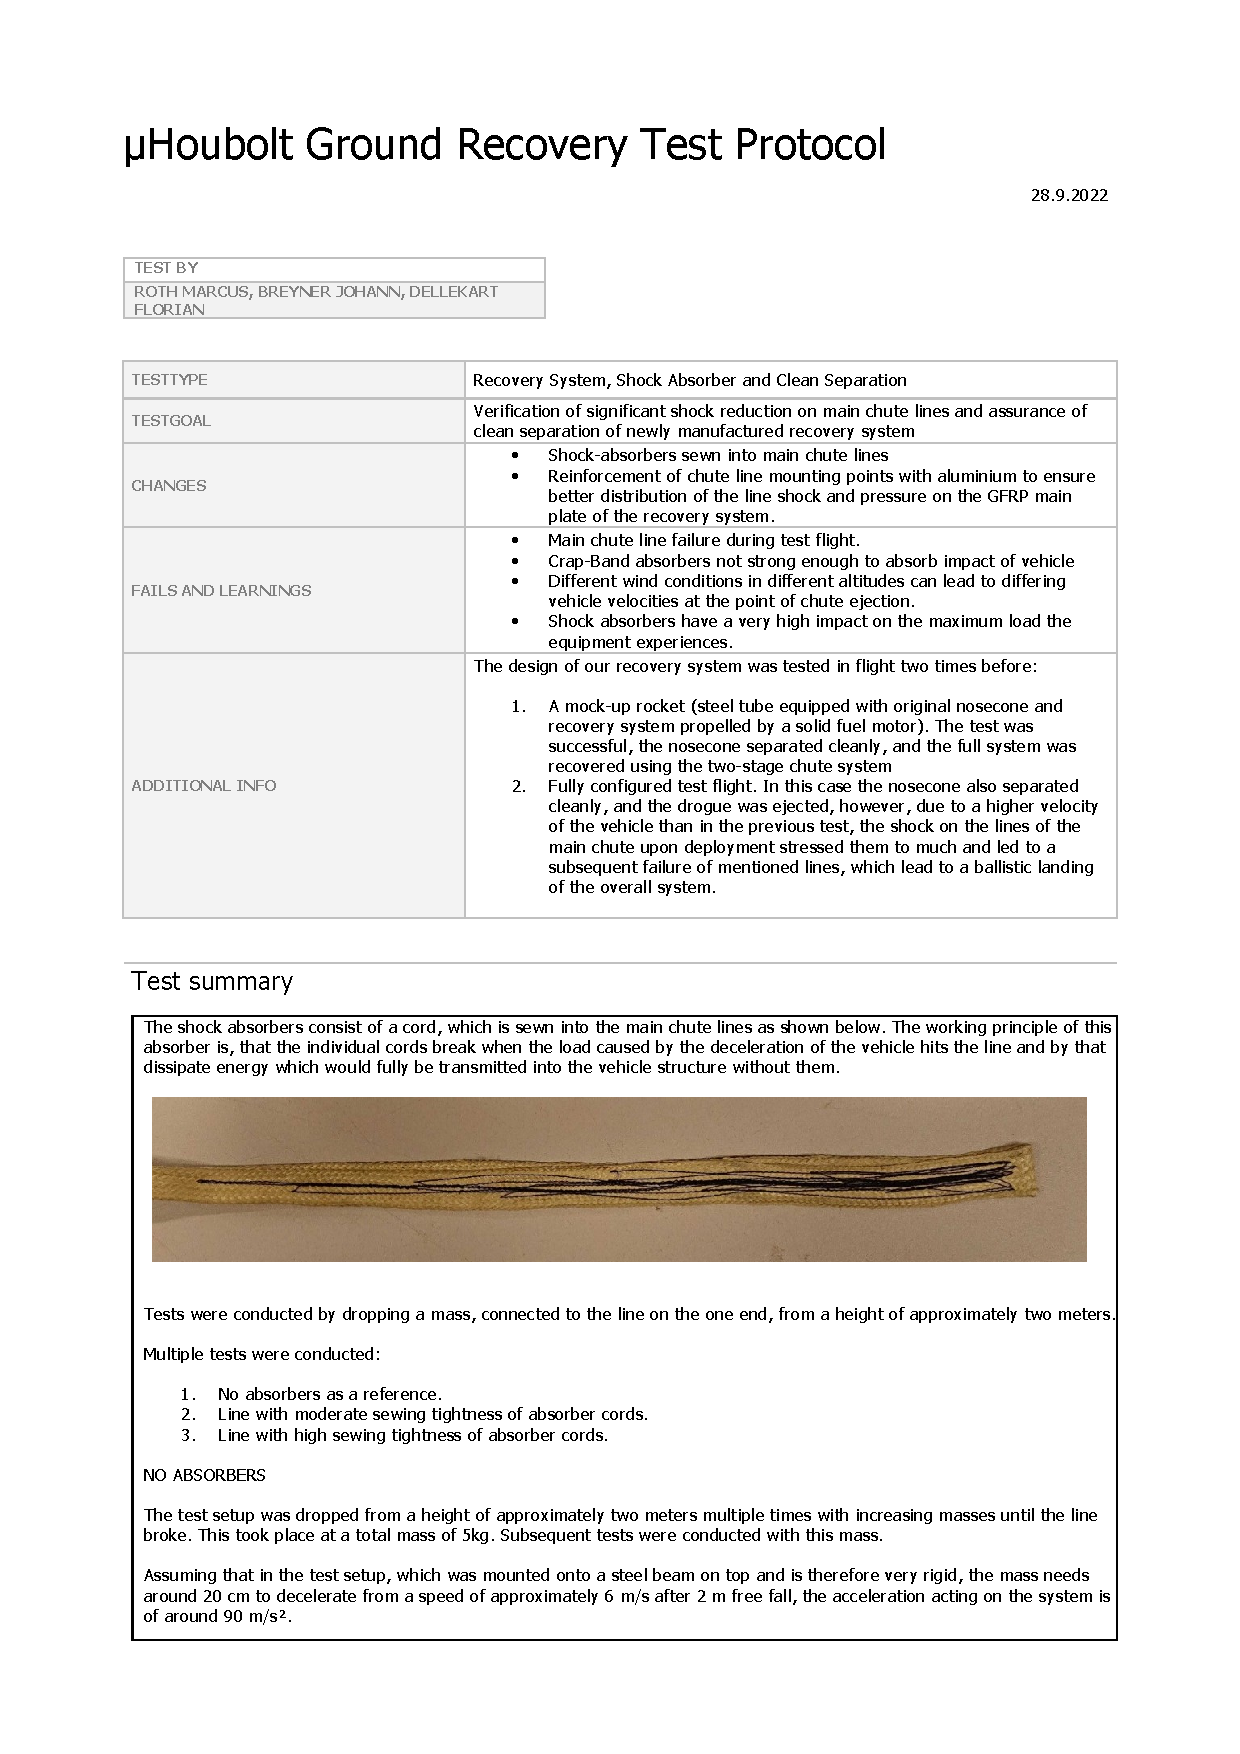
\includepdf[pages={1-4}]{Appendices/uHouboltRecoveryTestProtocol.pdf}

\newpage

\subsection{Flight Test Demonstration of Recovery System}

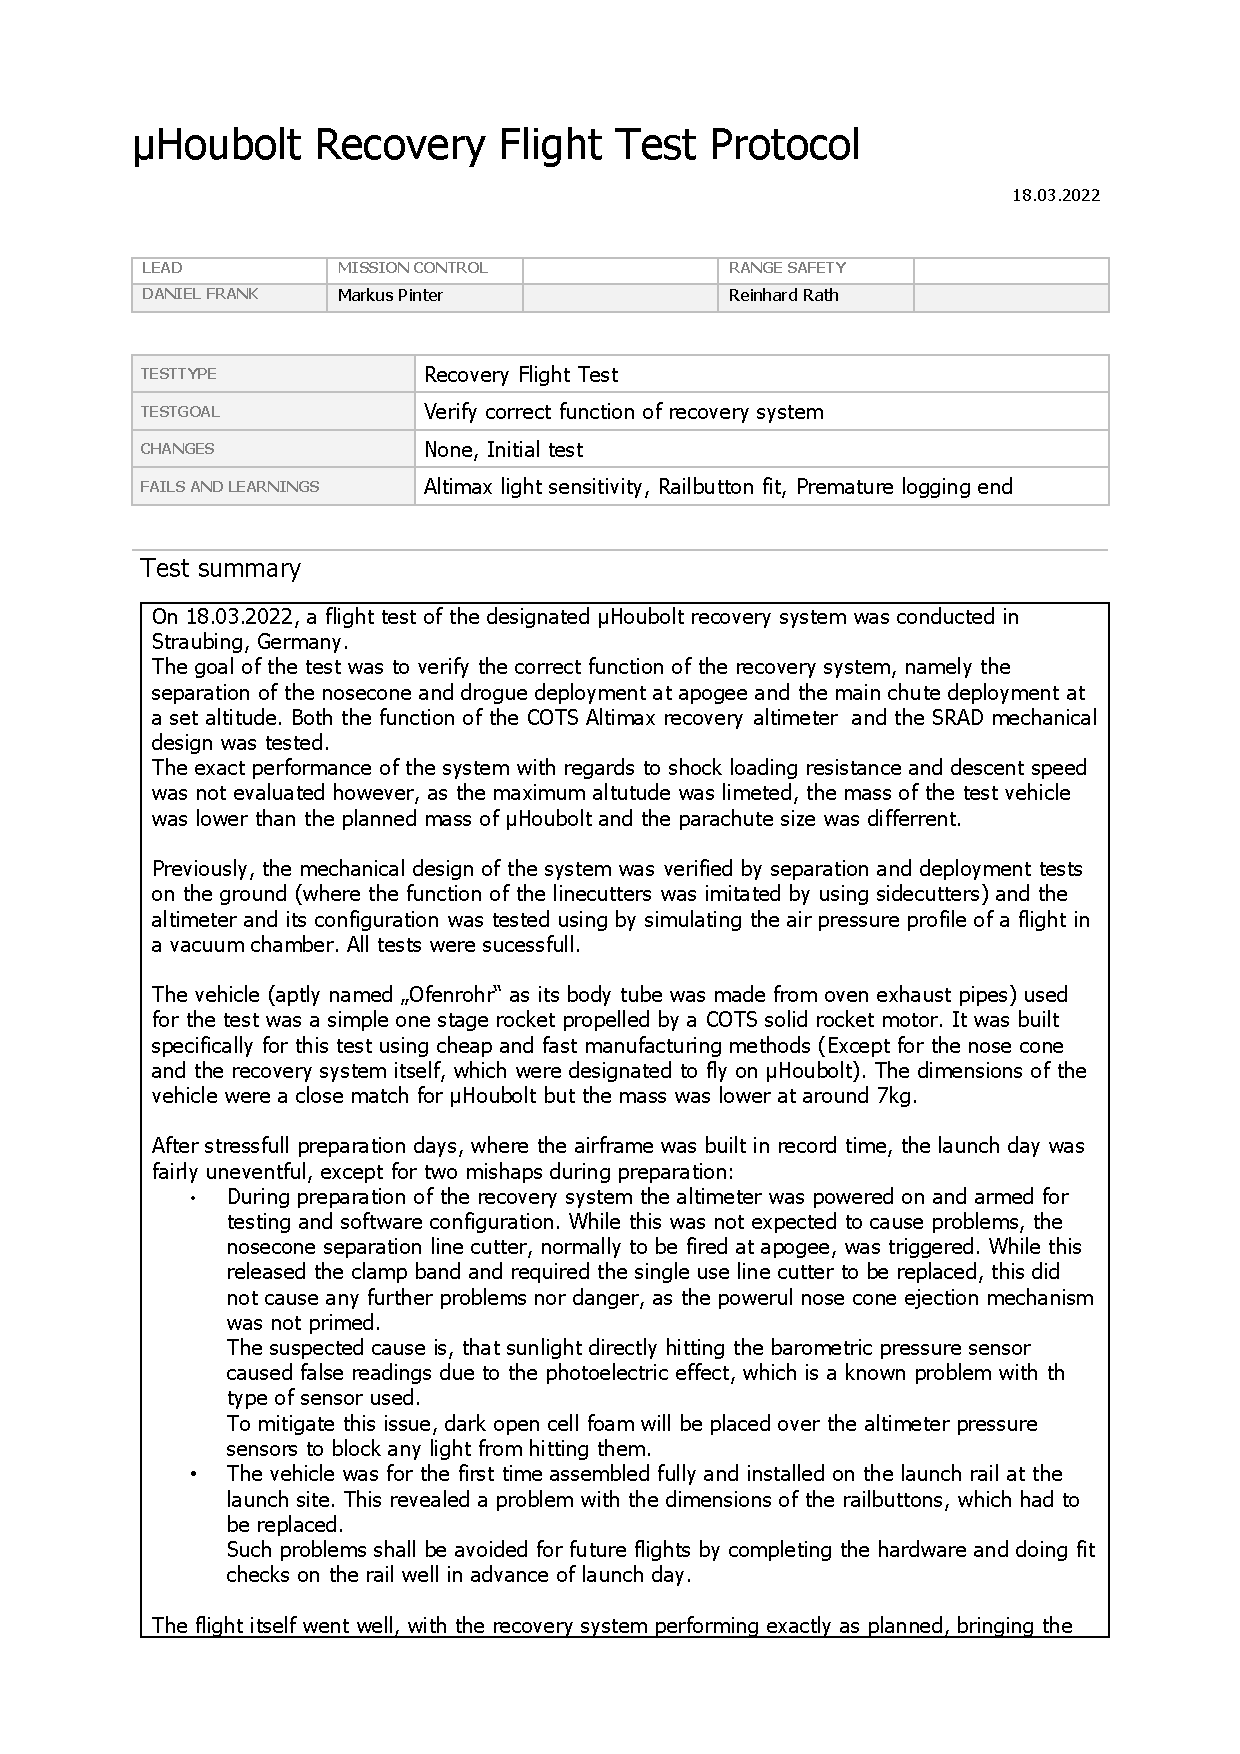
\includepdf[pages=-]{Appendices/uHoubolt_Recovery_Flight_Test_signed.pdf}

\subsection{Static Hot-Fire}

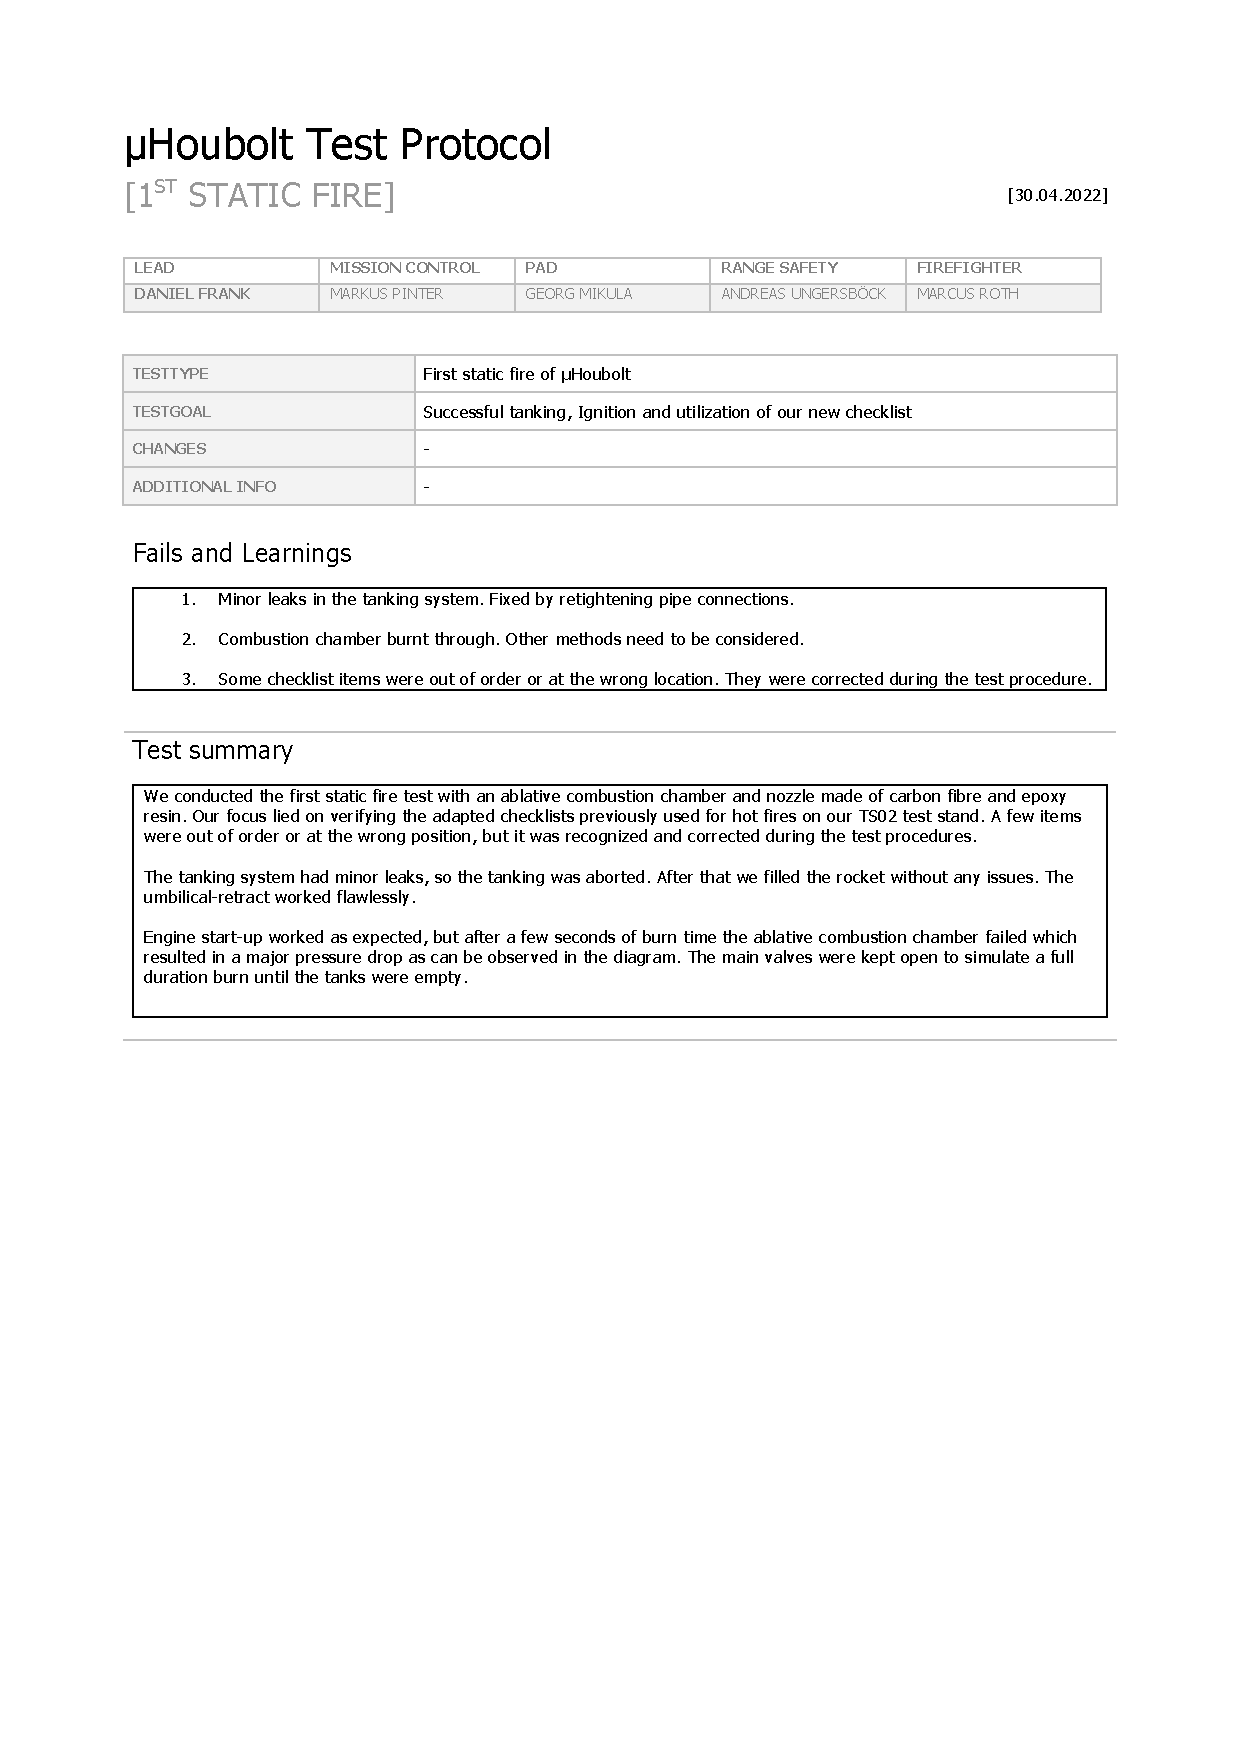
\includepdf[pages=-]{Appendices/uHoubolt_static_fire_220430_protocol.pdf}
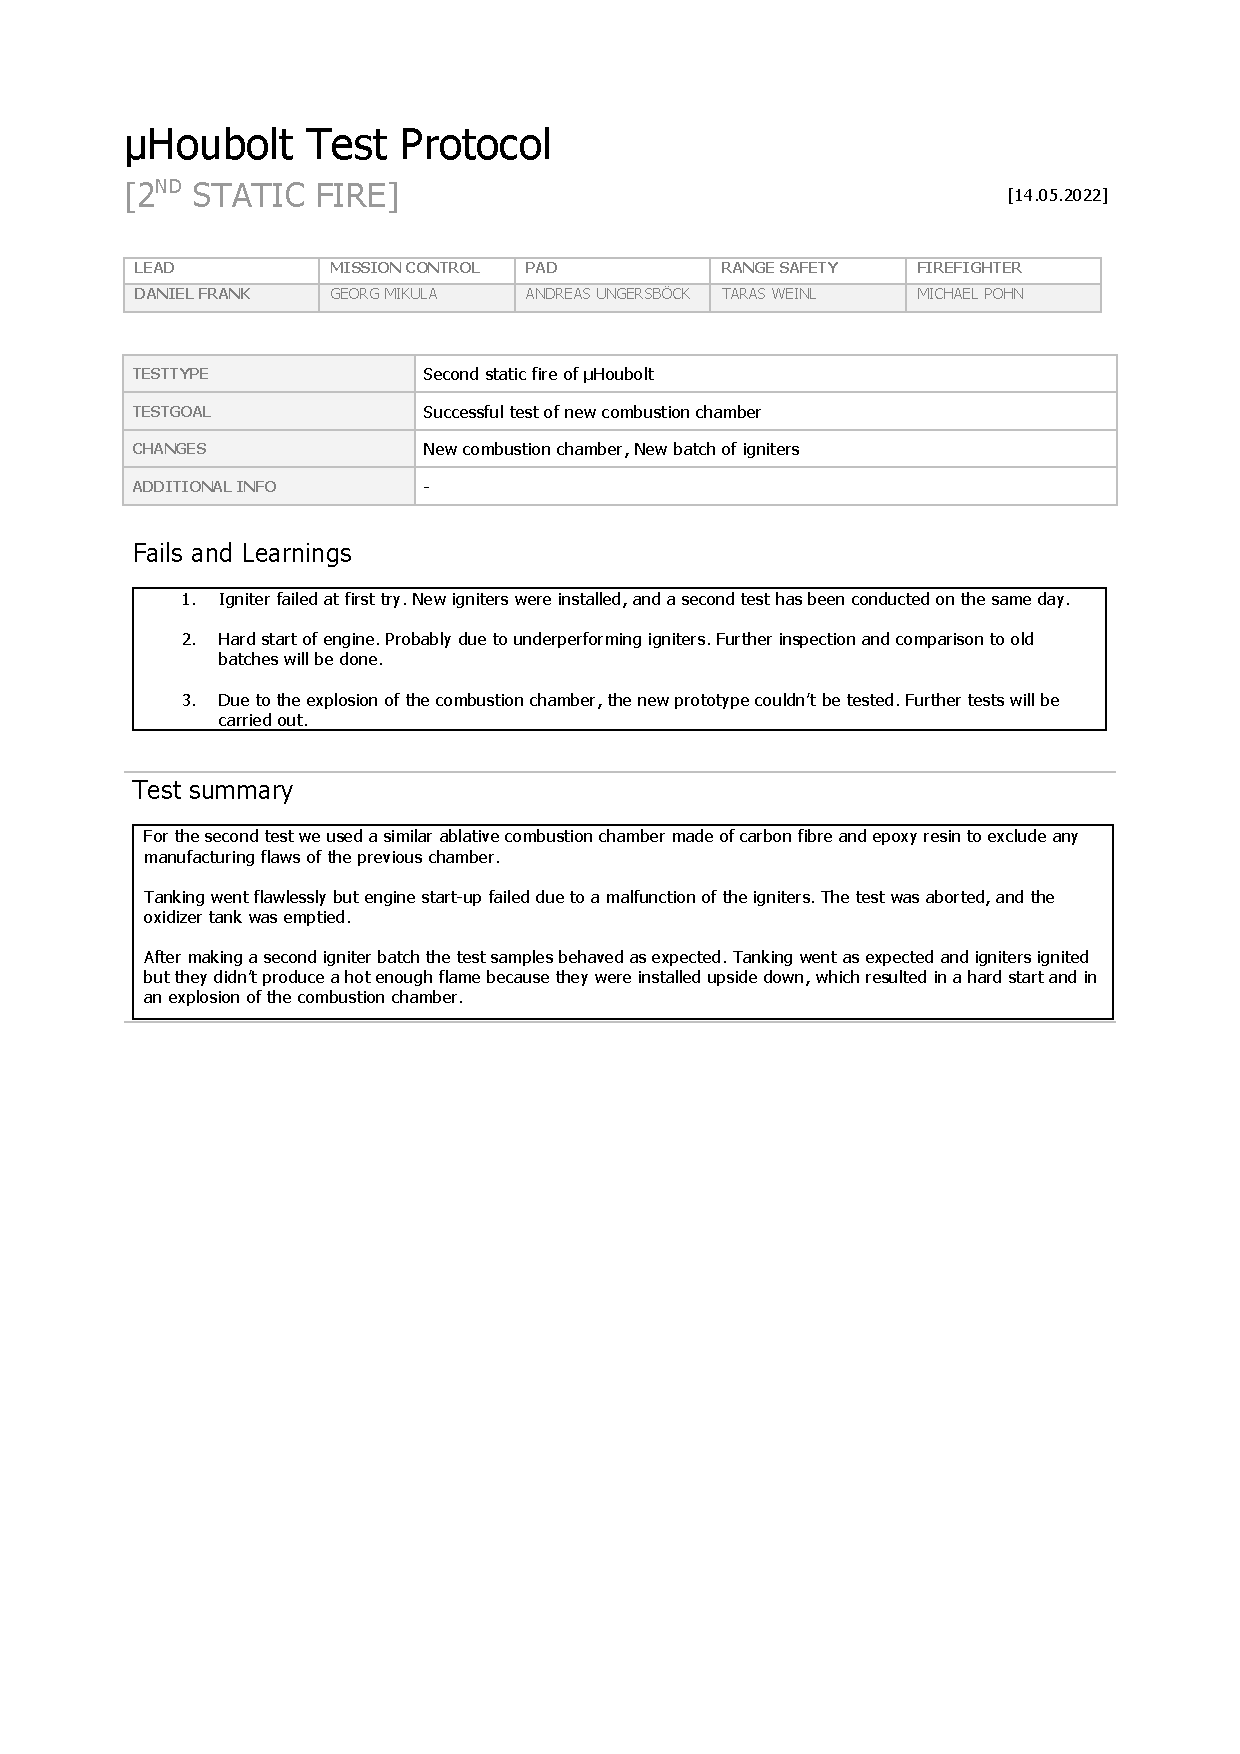
\includepdf[pages=-]{Appendices/uHoubolt_static_fire_220514_protocol.pdf}
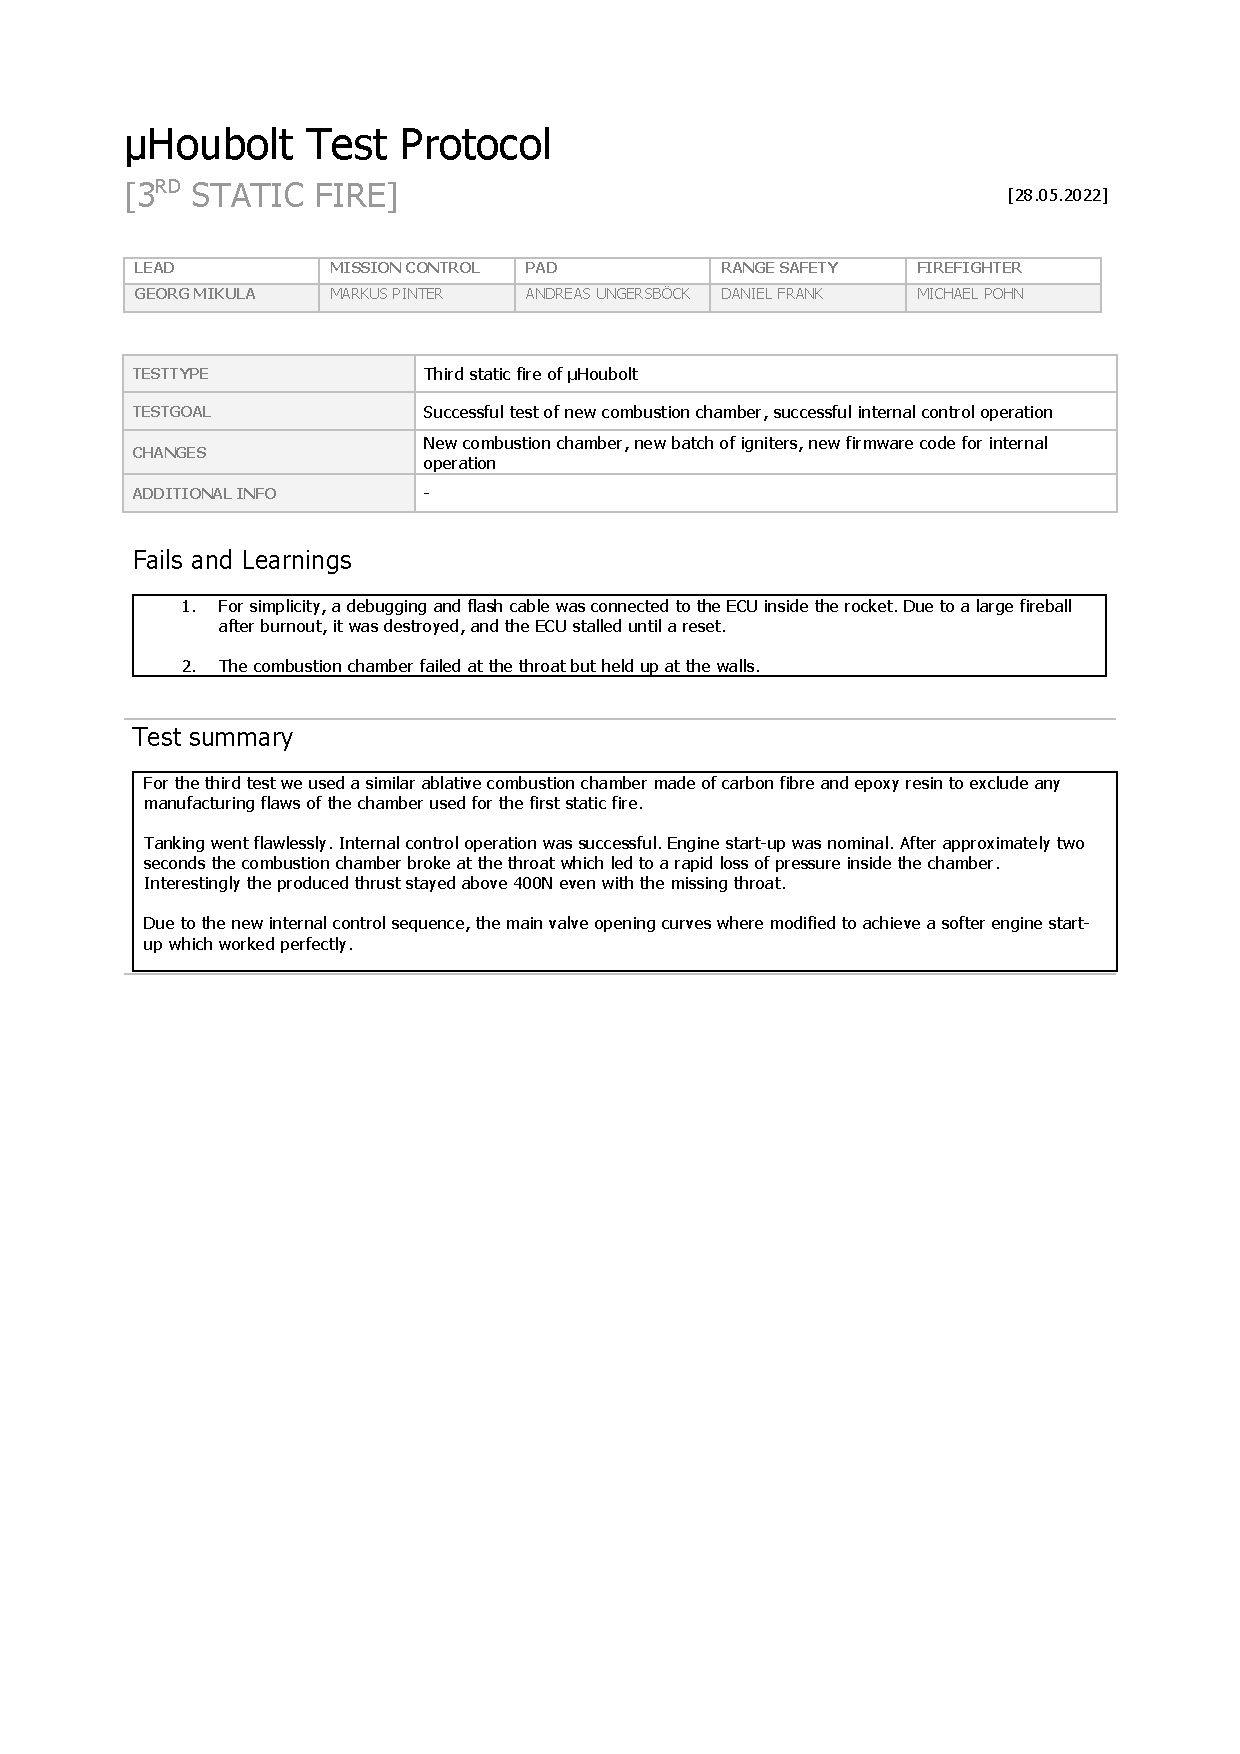
\includepdf[pages=-]{Appendices/uHoubolt_static_fire_220528_protocol.pdf}
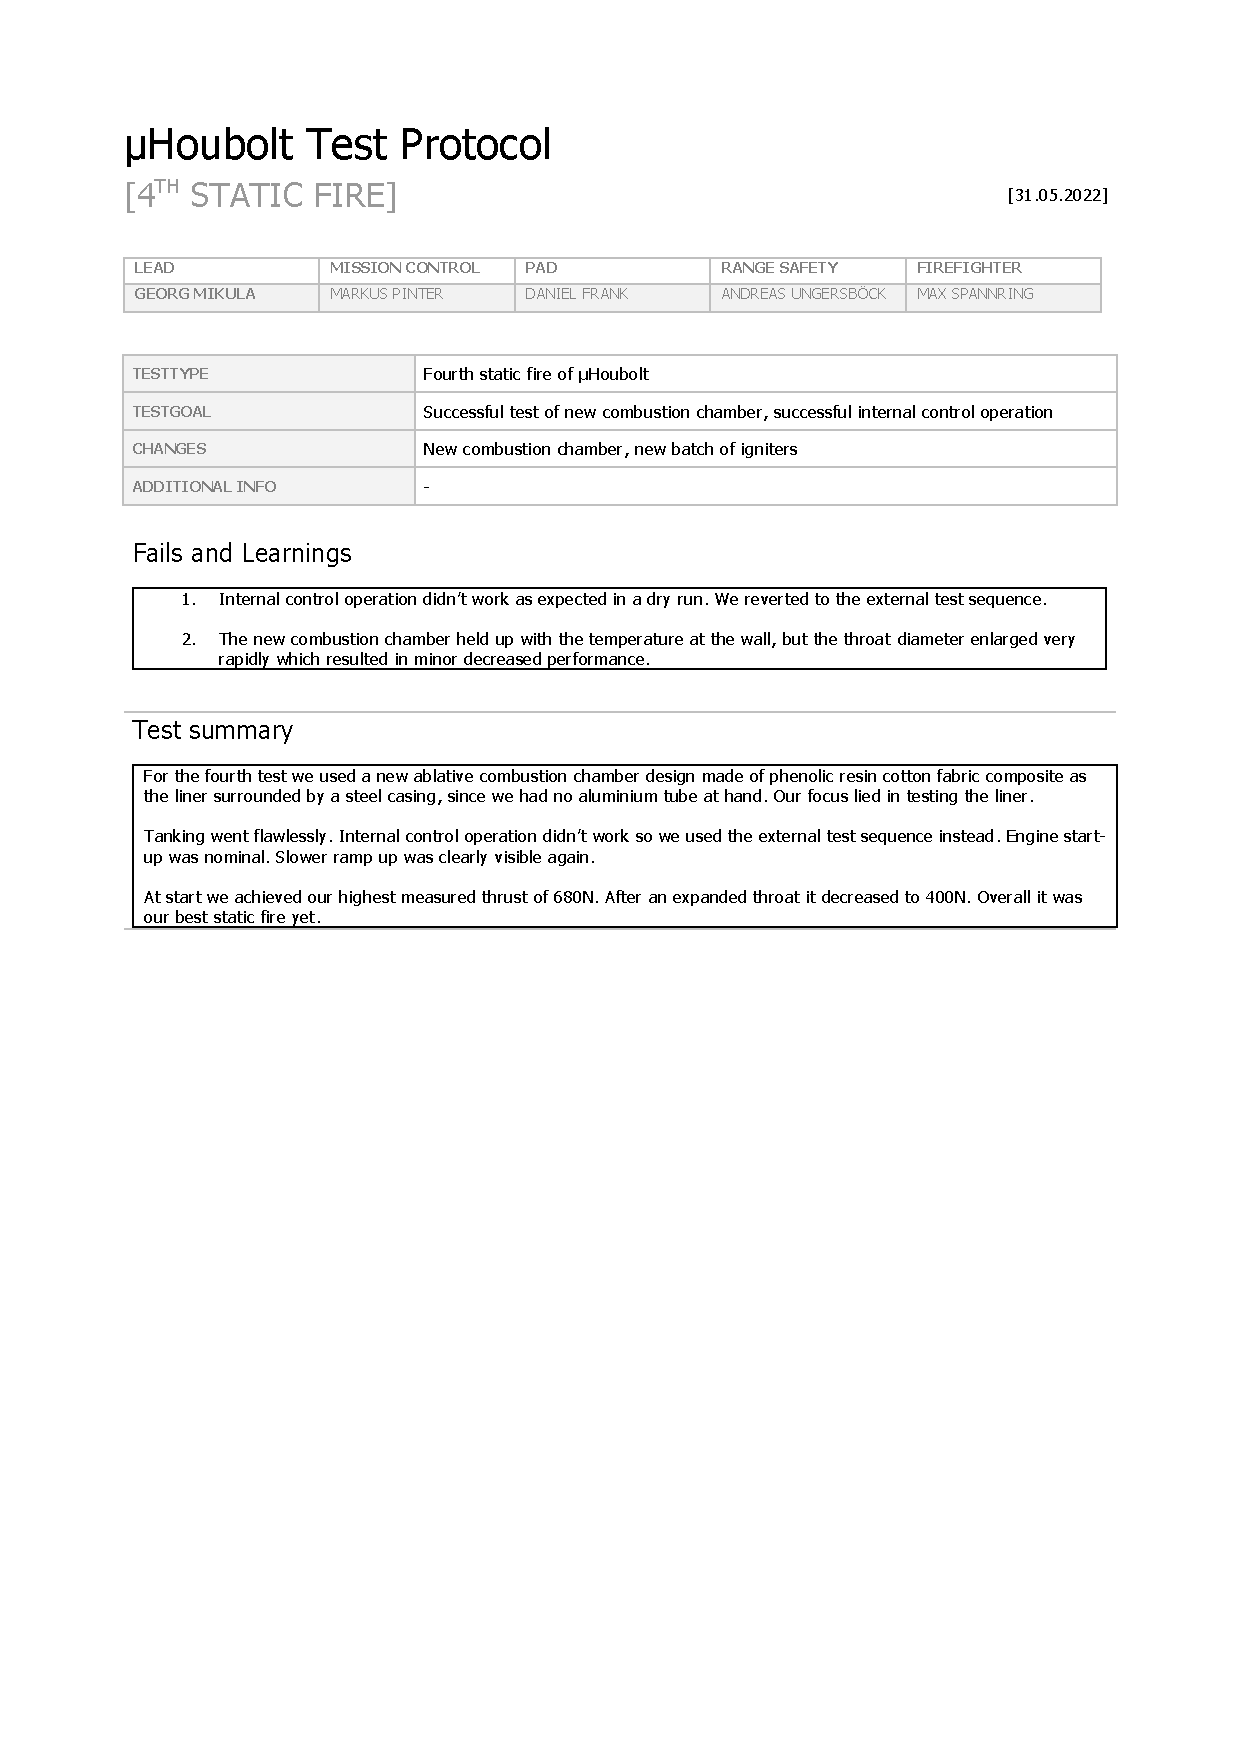
\includepdf[pages=-]{Appendices/uHoubolt_static_fire_220531_protocol.pdf}
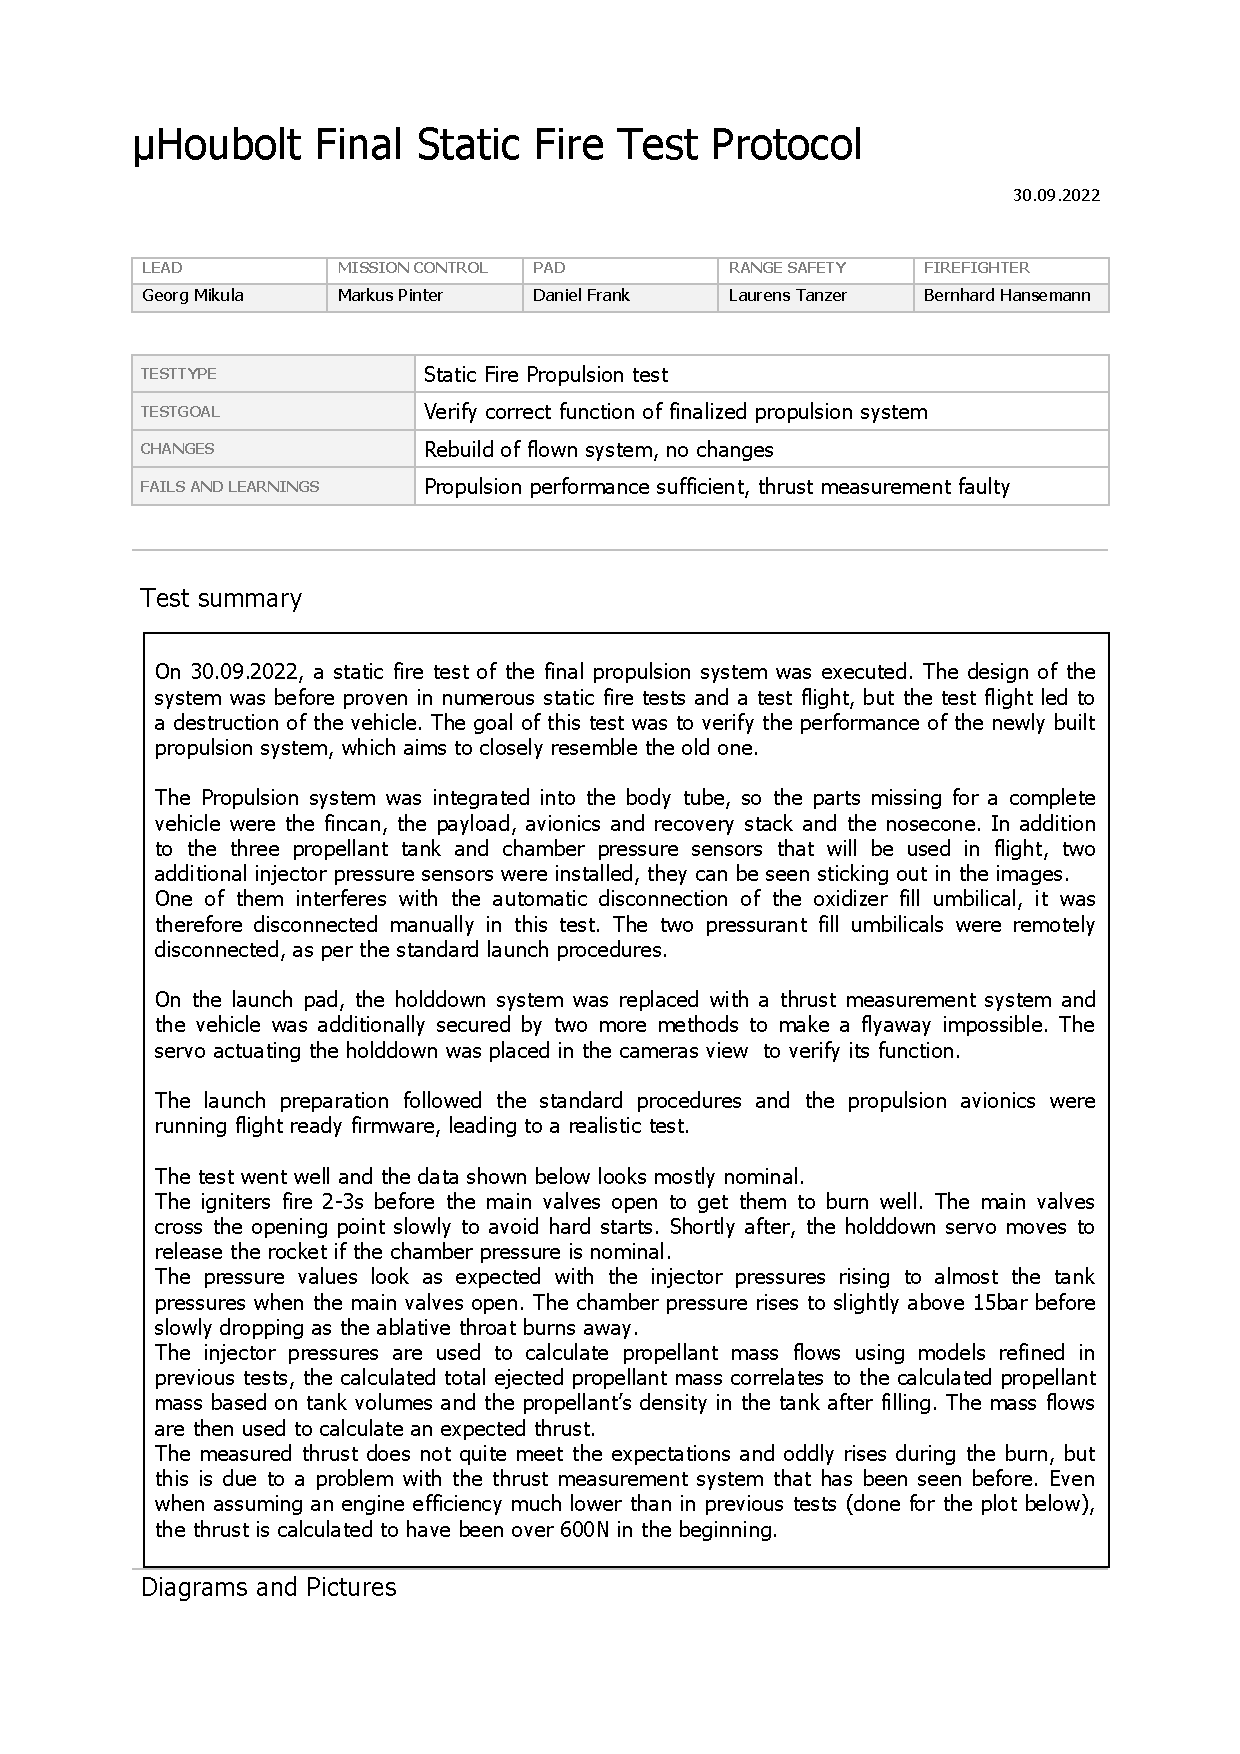
\includepdf[pages=-]{Appendices/uHoubolt_Static_Fire_Test_Protocol.pdf}

\subsection{Liquid Propellant loading and off-loading}

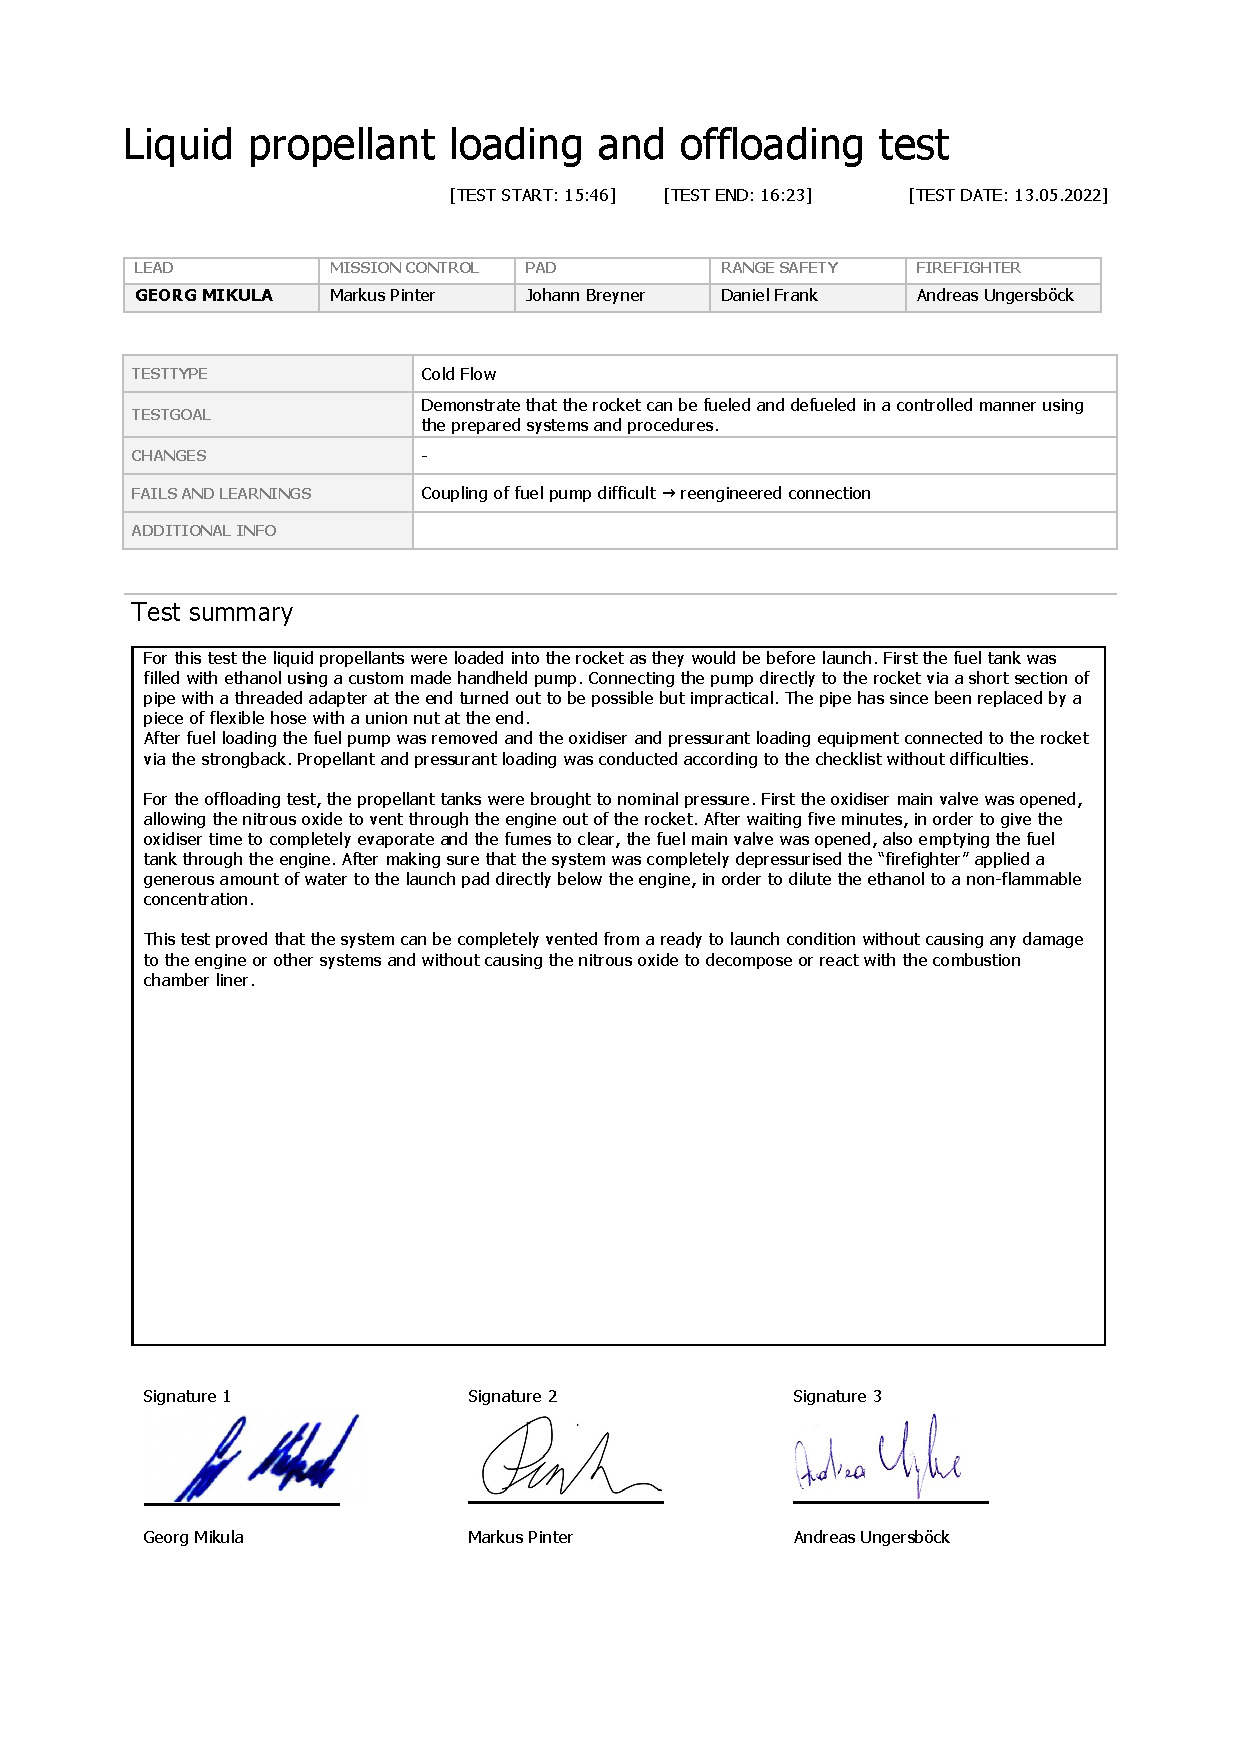
\includepdf[pages=-]{Appendices/uHoubolt_Loading_Offloading_signed.pdf}

\subsection{Combustion Chamber Pressure}

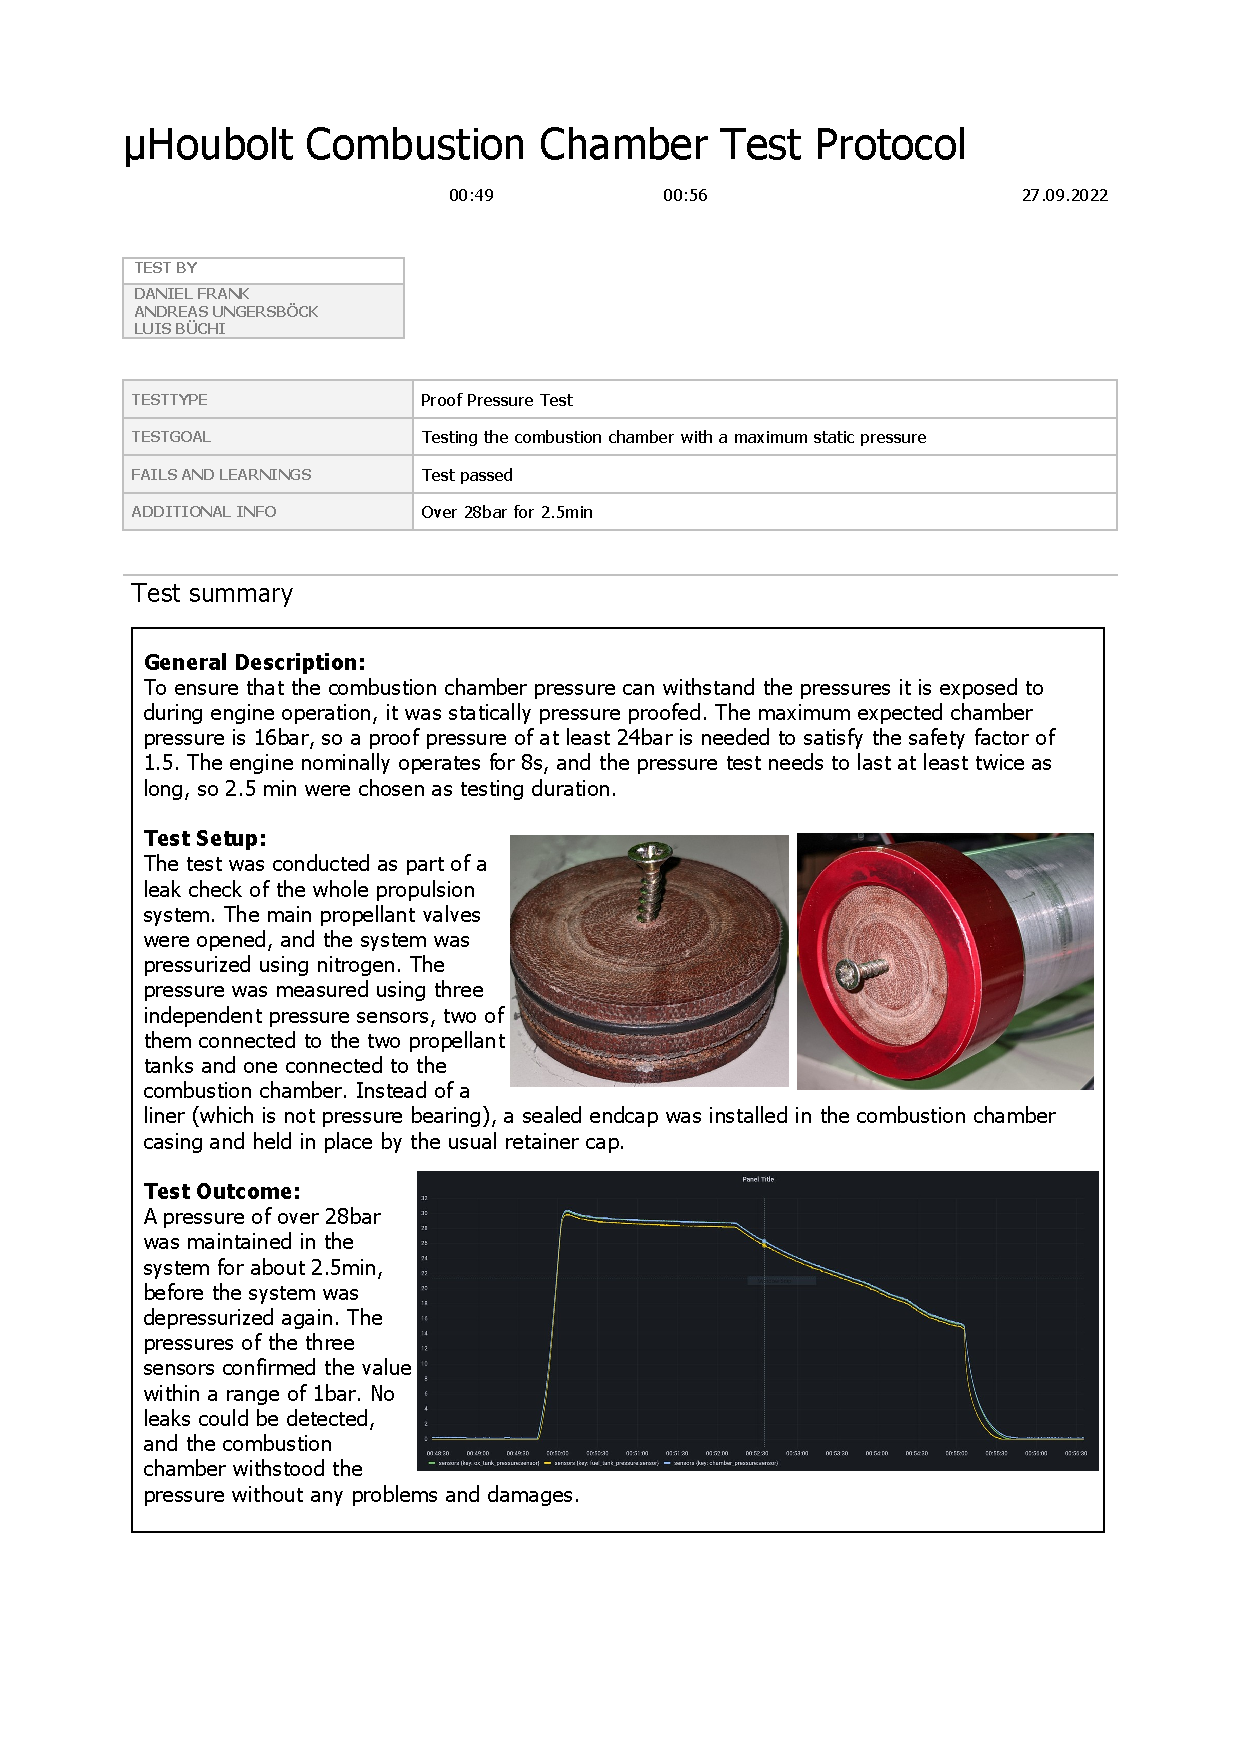
\includepdf[pages=-]{Appendices/uHoubolt_Combustion_Chamber_Test_Protocol.pdf}

\newpage

\subsection{Proof Pressure Testing Pressure Vessels}\label{sec:app_proof_pressure_testing}

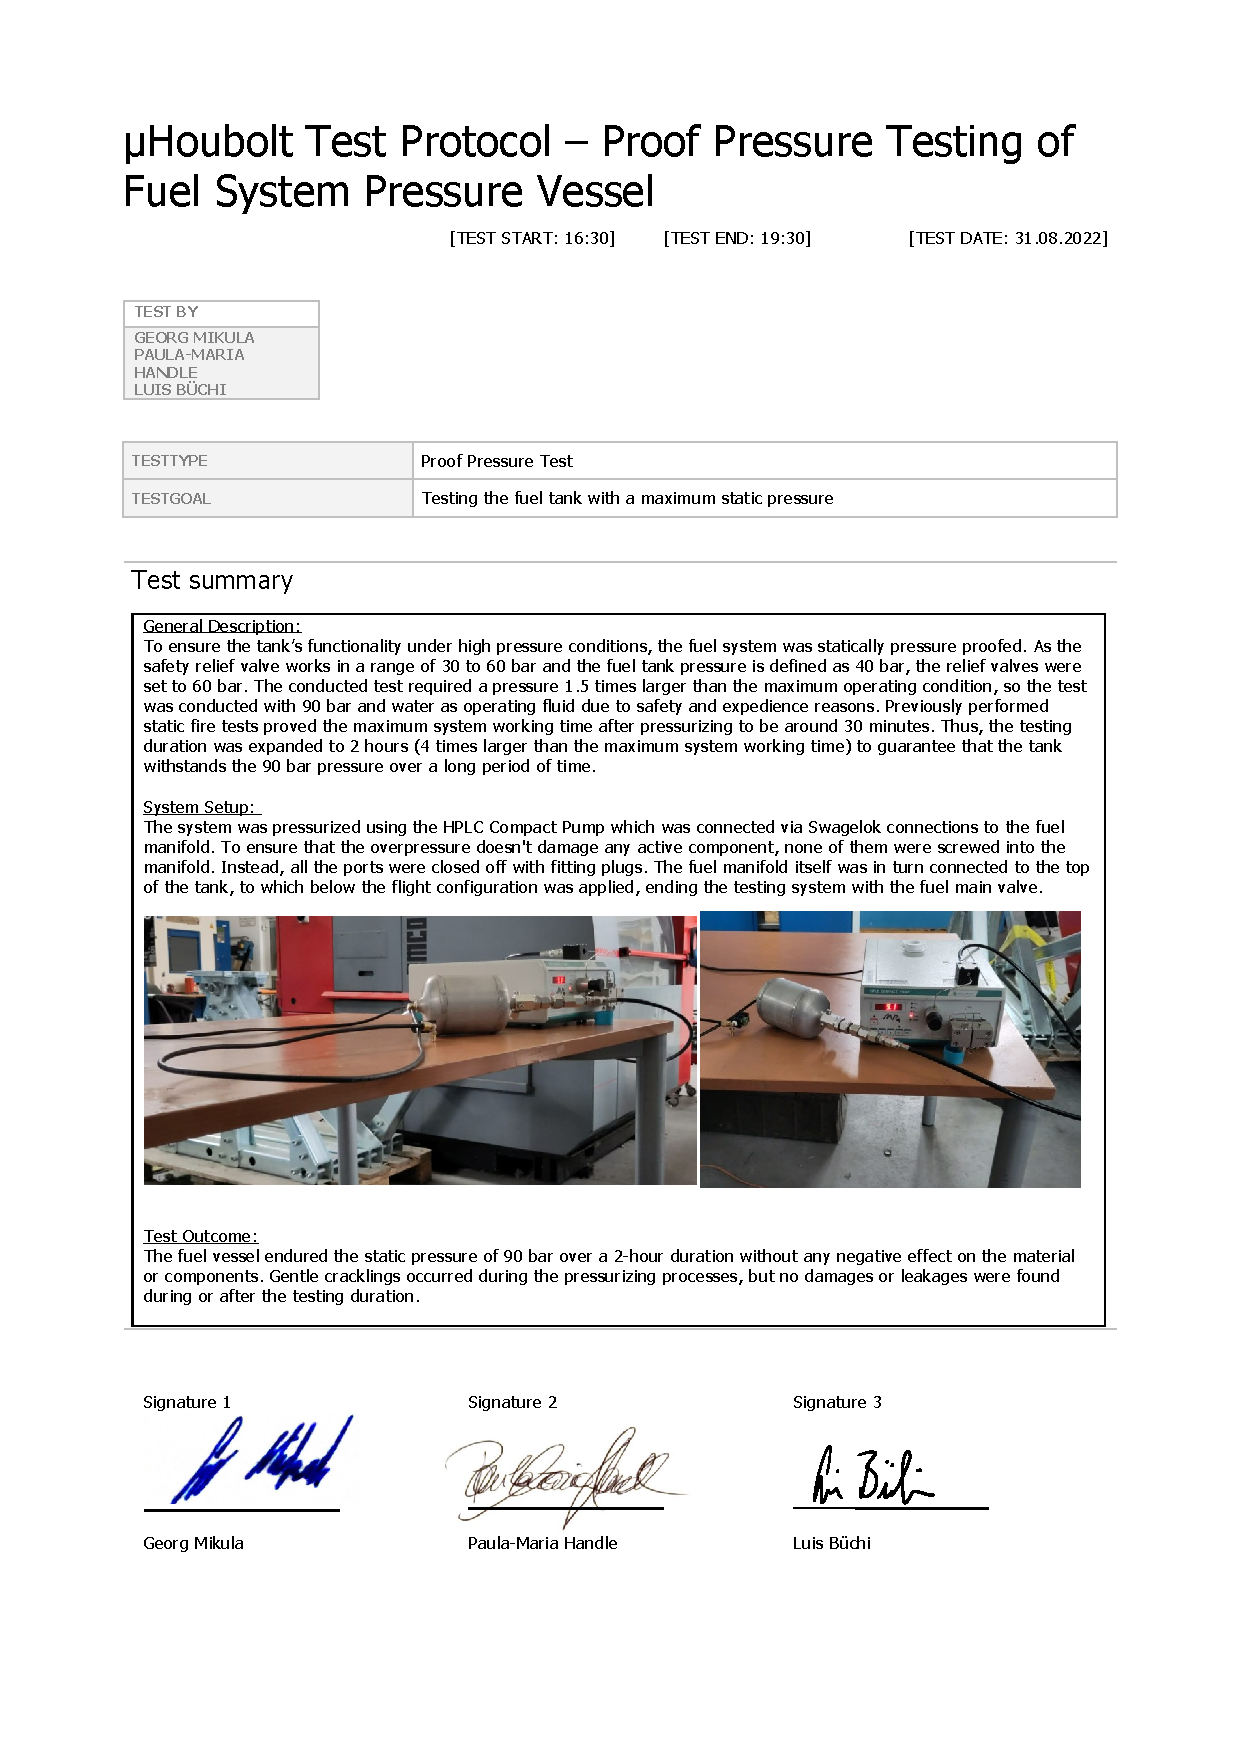
\includepdf[pages=-]{Appendices/uHoubolt_Proof_Pressure_Test_Fuel_Tank_signed.pdf}

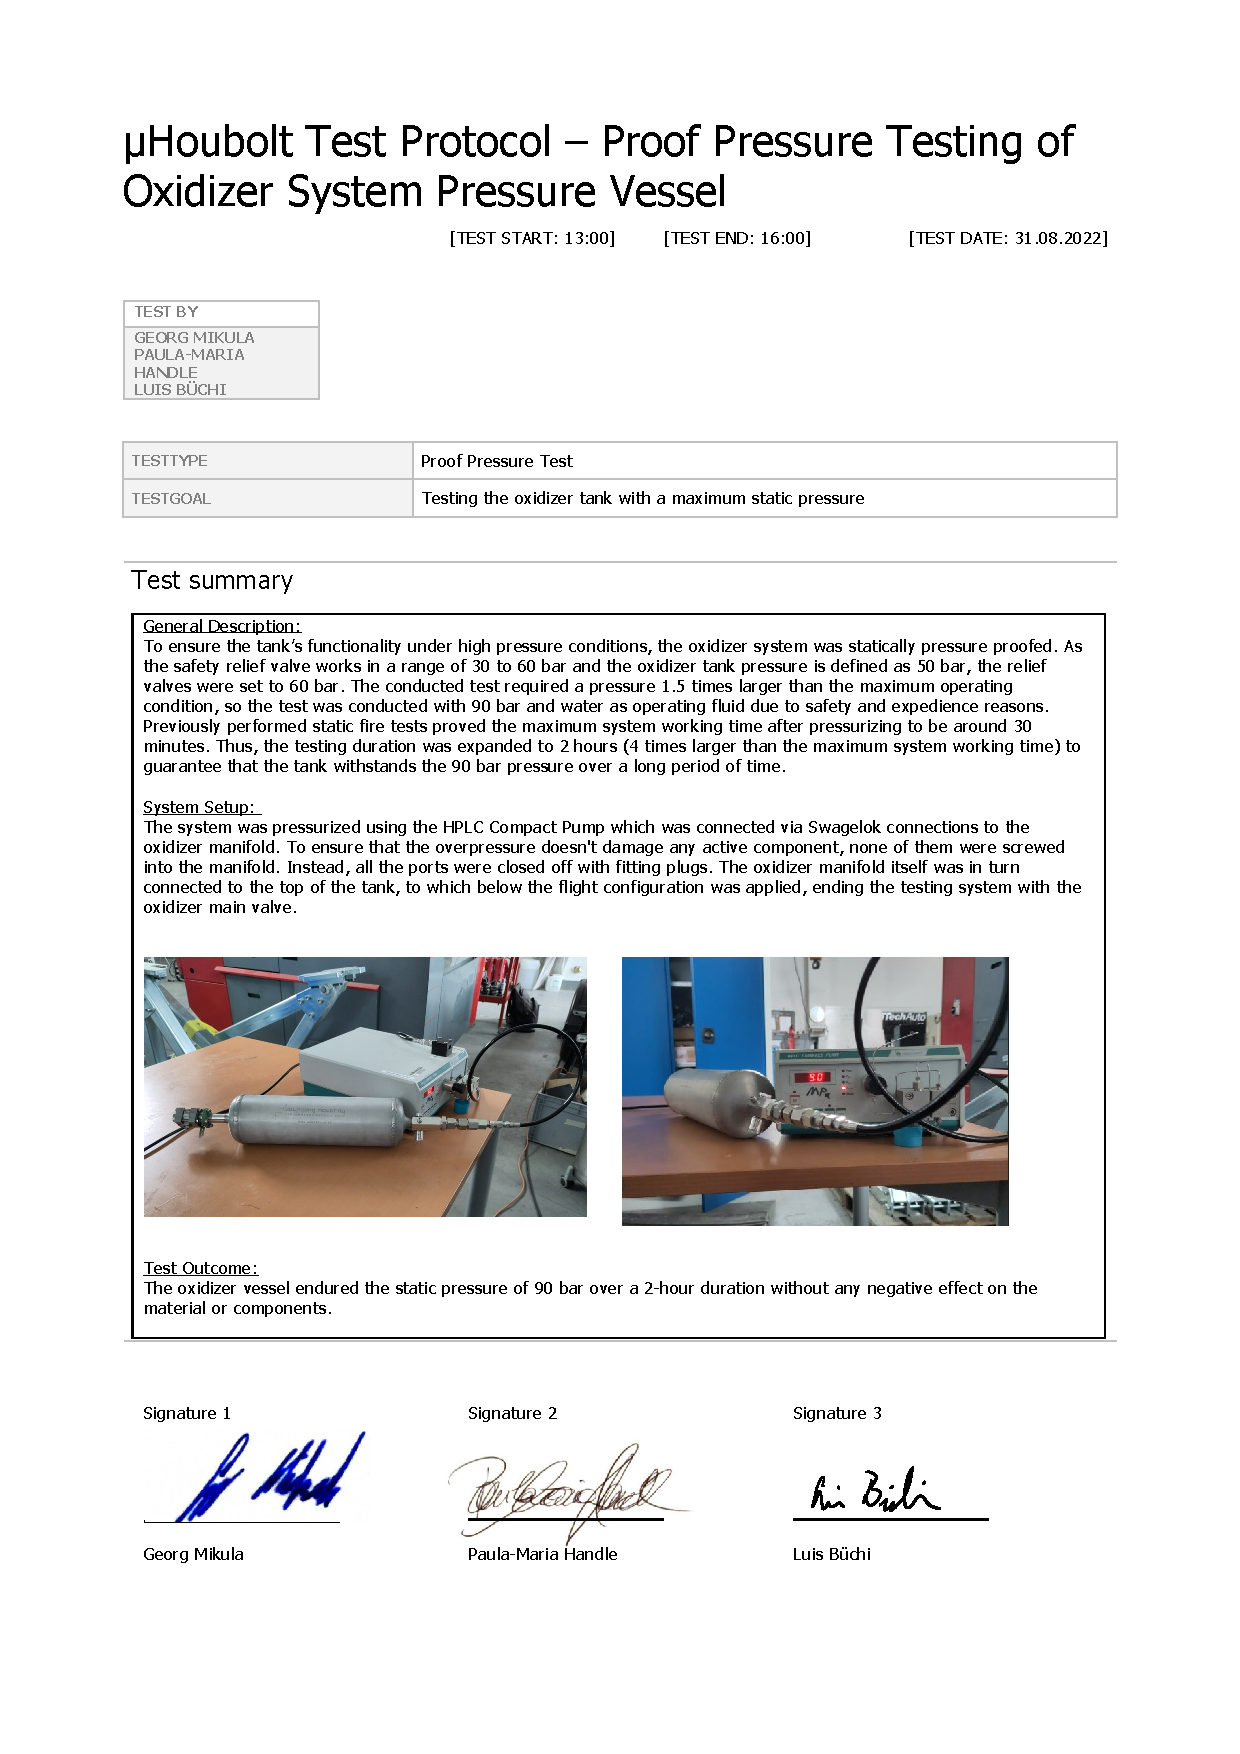
\includepdf[pages=-]{Appendices/uHoubolt_Proof_Pressure_Test_Ox_Tank_signed.pdf}

\subsection{Burst Pressure Testing Pressure Vessels}

THIS PAGE INTENTIONALLY LEFT BLANK

\newpage

\subsection{Test of SRAD flight computers with capability of actuating the recovery systems}

THIS PAGE INTENTIONALLY LEFT BLANK

\newpage

\section{Hazard Analysis Report}

\subsection{Liquid Propulsion System}

The liquid propulsion system contains by definition several hazardous materials and components:

\begin{itemize}
    \item Igniter
    \item Ethanol
    \item Nitrous Oxide
\end{itemize}

In the following the hazards related to these materials and the mitigations for them are laid out.

\begin{itemize}
    \item Transport
    \begin{itemize}
        \item \textbf{Igniter}
        
        Hazard: As the igniter is unsurprisingly flammable it poses a risk of starting to burn at an unwanted time. 
        
        Mitigation: The igniter mixture is put together on premise shortly before needing it, during transport the individual components are not dangerous.
        
        \item \textbf{Ethanol}
        
        Hazard: While not burning quickly, Ethanol is flammable and evaporates quickly.
        
        Mitigation: The ethanol gets transported and stored in their original packaging (plastic bottles).
        
        \item \textbf{Nitrous Oxide}
        
        Hazard: Tipping over could break the bottle open.
        
        Mitigation: Only gets transported with the safety lid on.
    \end{itemize}
\end{itemize}

\begin{itemize}
    \item Usage
    \begin{itemize}
        \item \textbf{Igniter}
        
        Hazard: Igniter going off after being installed on the combustion chamber or while being manufactured.
        
        Mitigation: The ignition system is only armed once the RBF pin is fully removed from the PMU, which happens just before launch preparations are done and the team vacates the launch pad. Before then, even on a misfire in the electronics, the igniter voltage to start the burning is physically disconnected. The person manufacturing the igniters wears eye protection and gloves. The heating plate is closely monitored to ensure proper heating temperature. All other people not involved hold their distance.
        
        \item \textbf{Ethanol}
        
        Hazard: Ethanol spills during handling could pose a fire risk on and around the pad.
        
        Mitigation: The ethanol gets filled into a large syringe away from the pad and then pushed from the syringe into the fuel tank. This removes potential spills from the pad.
        
        \item \textbf{Nitrous Oxide}
        
        Hazard: The nitrous oxide can explosively decompose.
        
        Mitigation: All parts that get in touch with the N2O get rigorously ox-cleaned. Filling the N2O tank in the rocket is one of the last steps of the launch checklist just before launch. Just one experienced member of personnel is at the launch rail. He/She opens the N2O gas cylinder. After some checks the last person leaves the launch rail. Only then the tanking of the N2O begins, controlled remotely from Mission Control. See \cref{sec:oxidizer_loading} for details on the oxidizer loading procedure.
    \end{itemize}
\end{itemize}

\subsection{Slingshot Mechanism in Recovery System}

Hazard: The slingshot mechanism of the recovery system stores considerable potential energy when loaded (See \cref{sec:recovery}). During launch preparations this has to be done a while before the pad crew vacates the premises and as such the slingshot mechanism could (mis)fire when personnel is around. This could happen if the knot loosens or the recovery system fails and prematurely detects apogee on the pad.

Mitigation: As soon as the mechanism is loaded a cable tie gets wrapped around the clampband which stops the mechanism from firing until removed right before the crew leaves the launch pad.

\section{Risk Assessment}

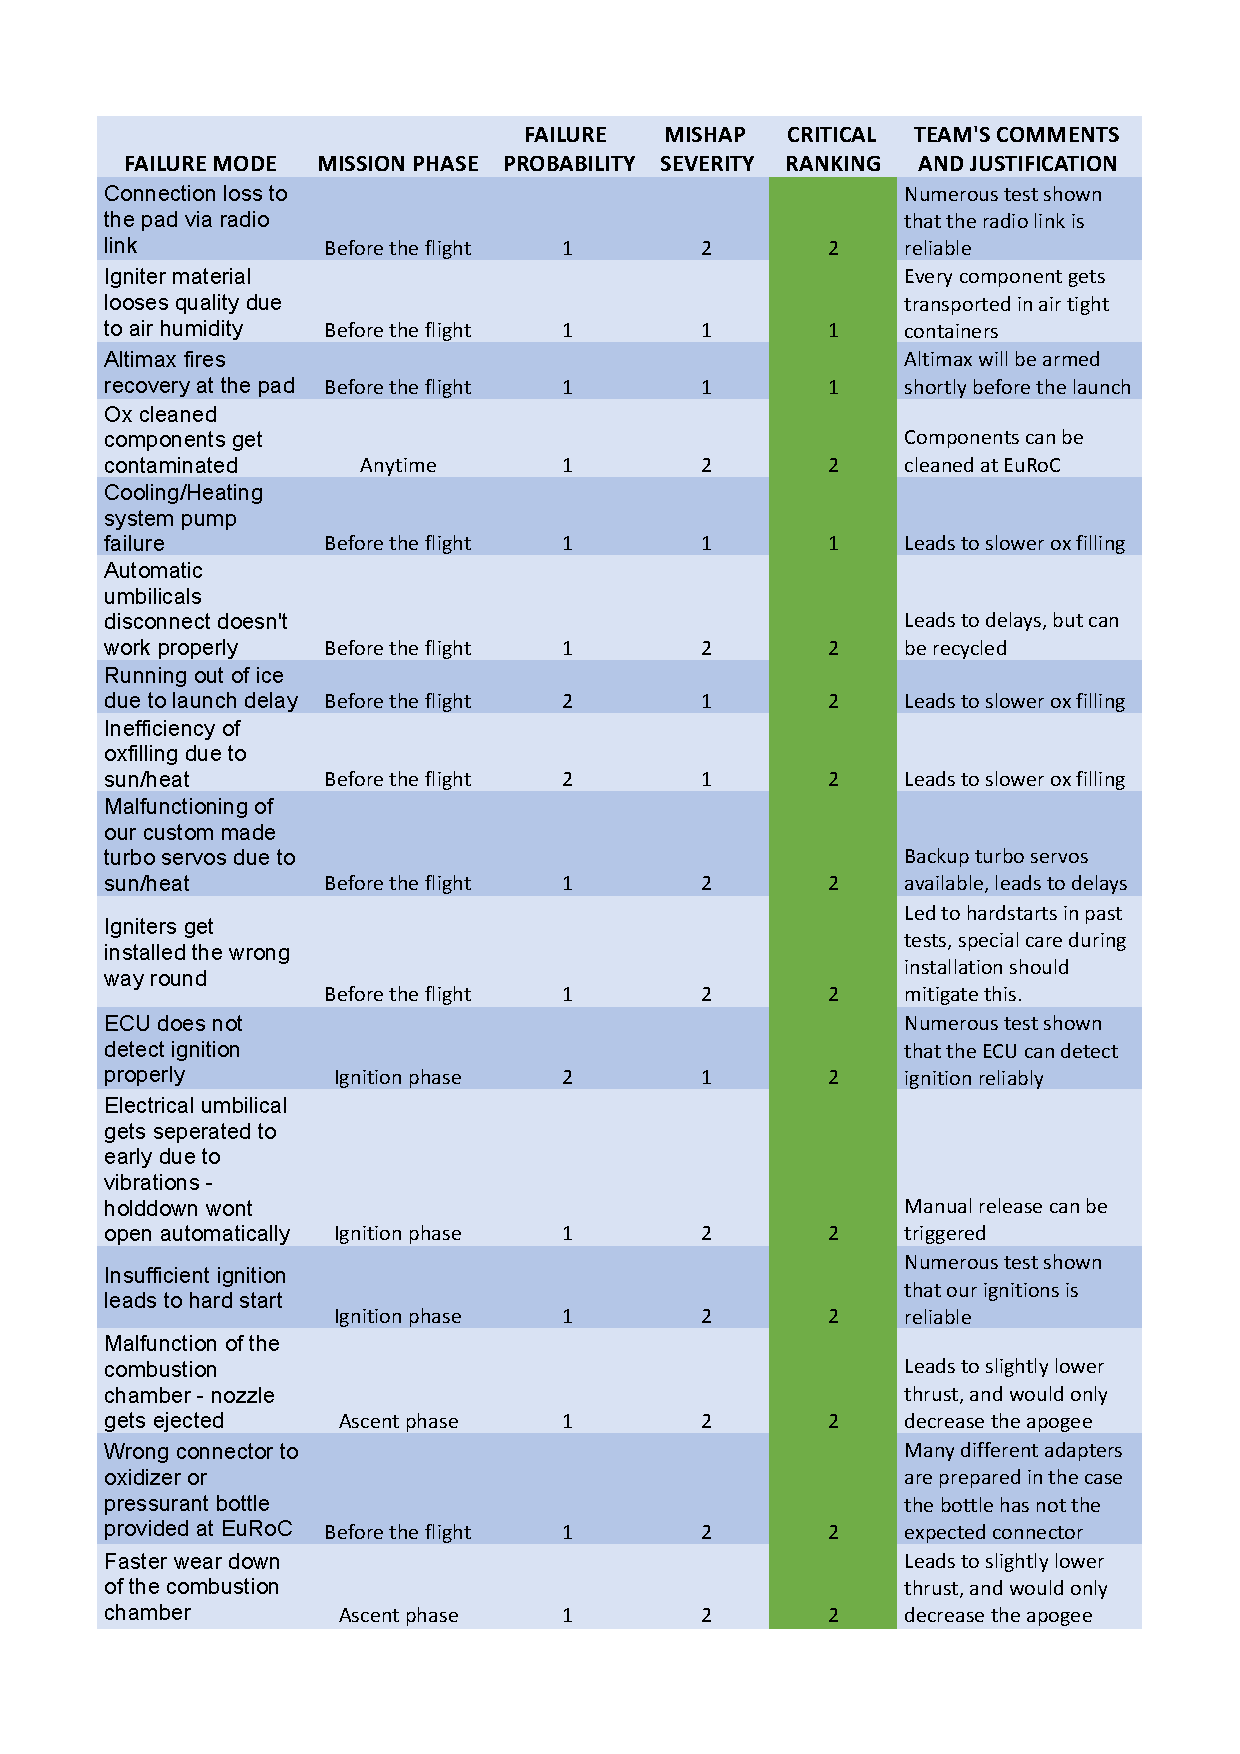
\includepdf[pages=-]{Appendices/RiskAssessment.pdf}

\section{Checklists}

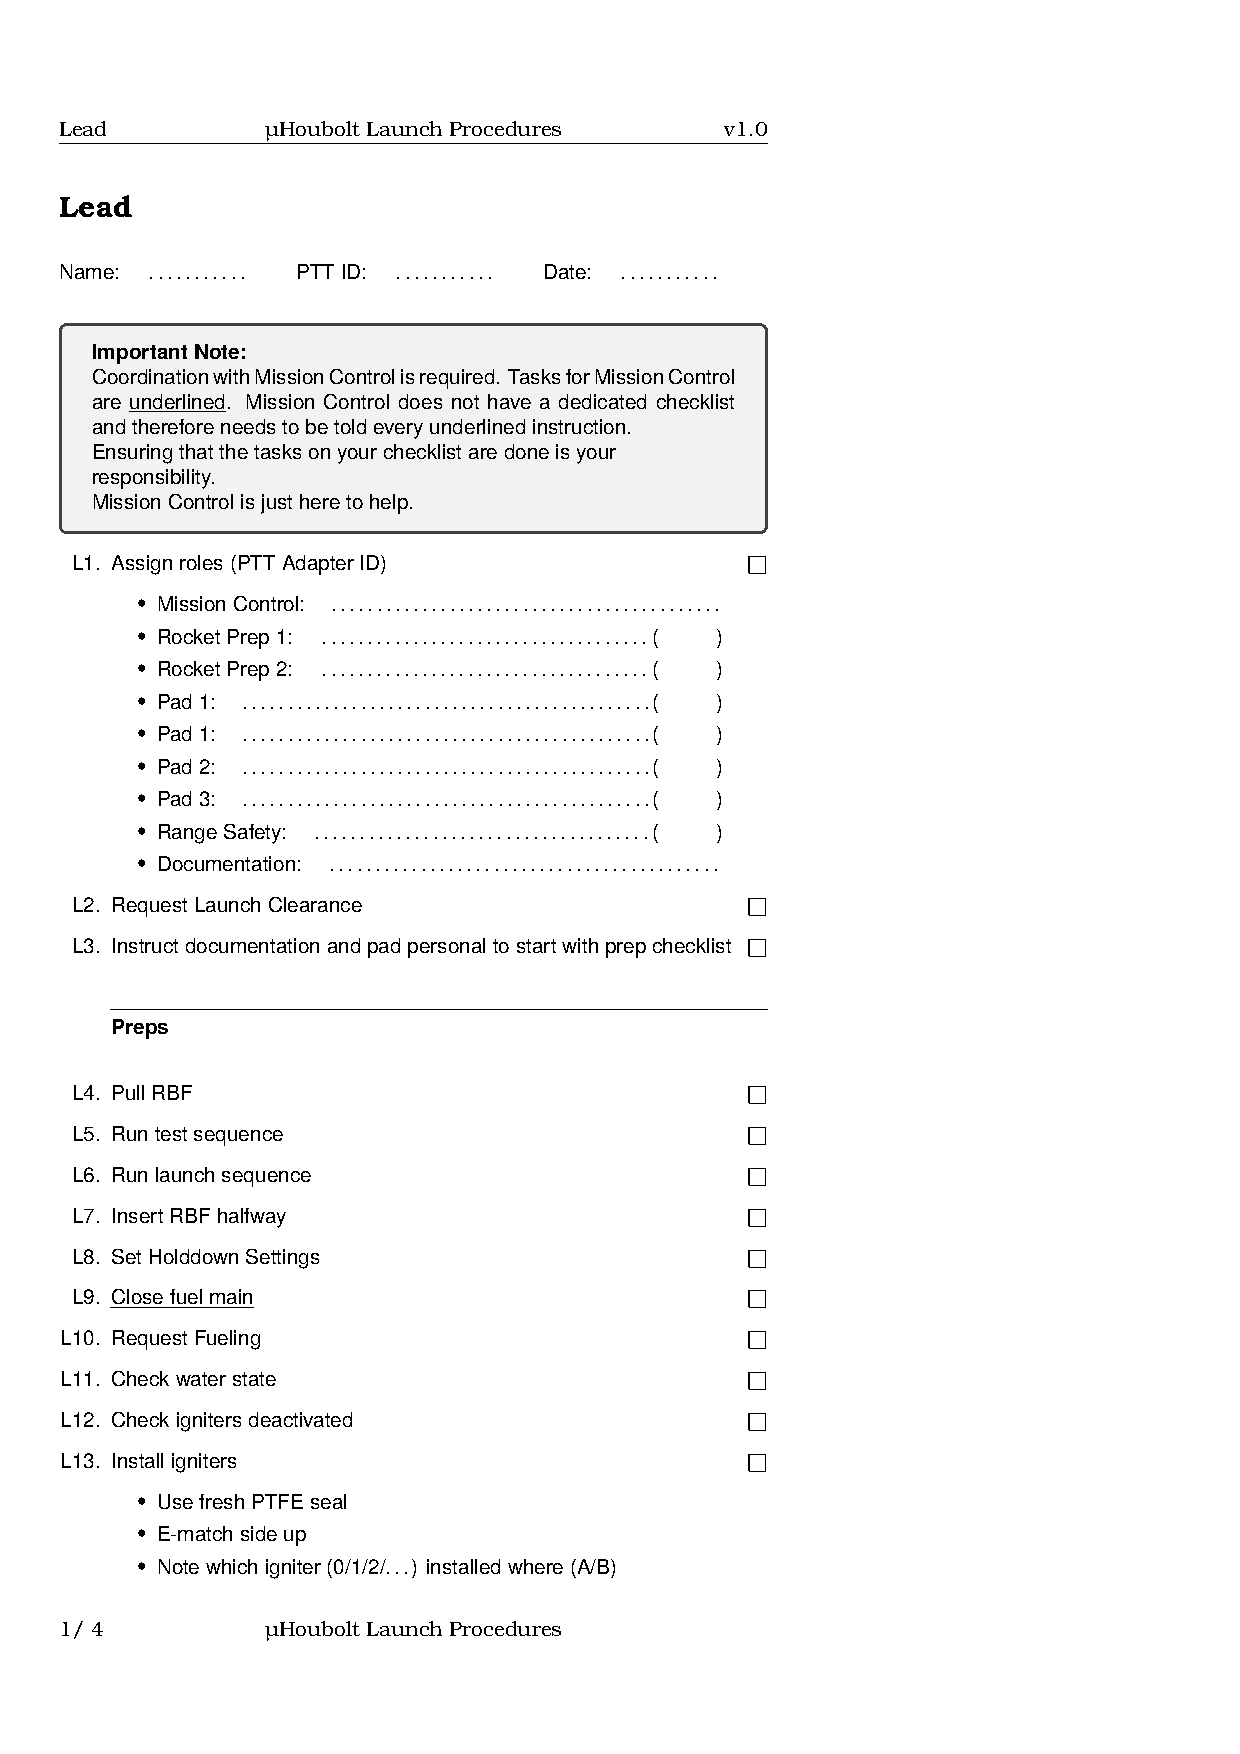
\includepdf[pages={1-6}]{Appendices/Houbolt_Launch_Procedures.pdf}

\section{Engineering Drawings}

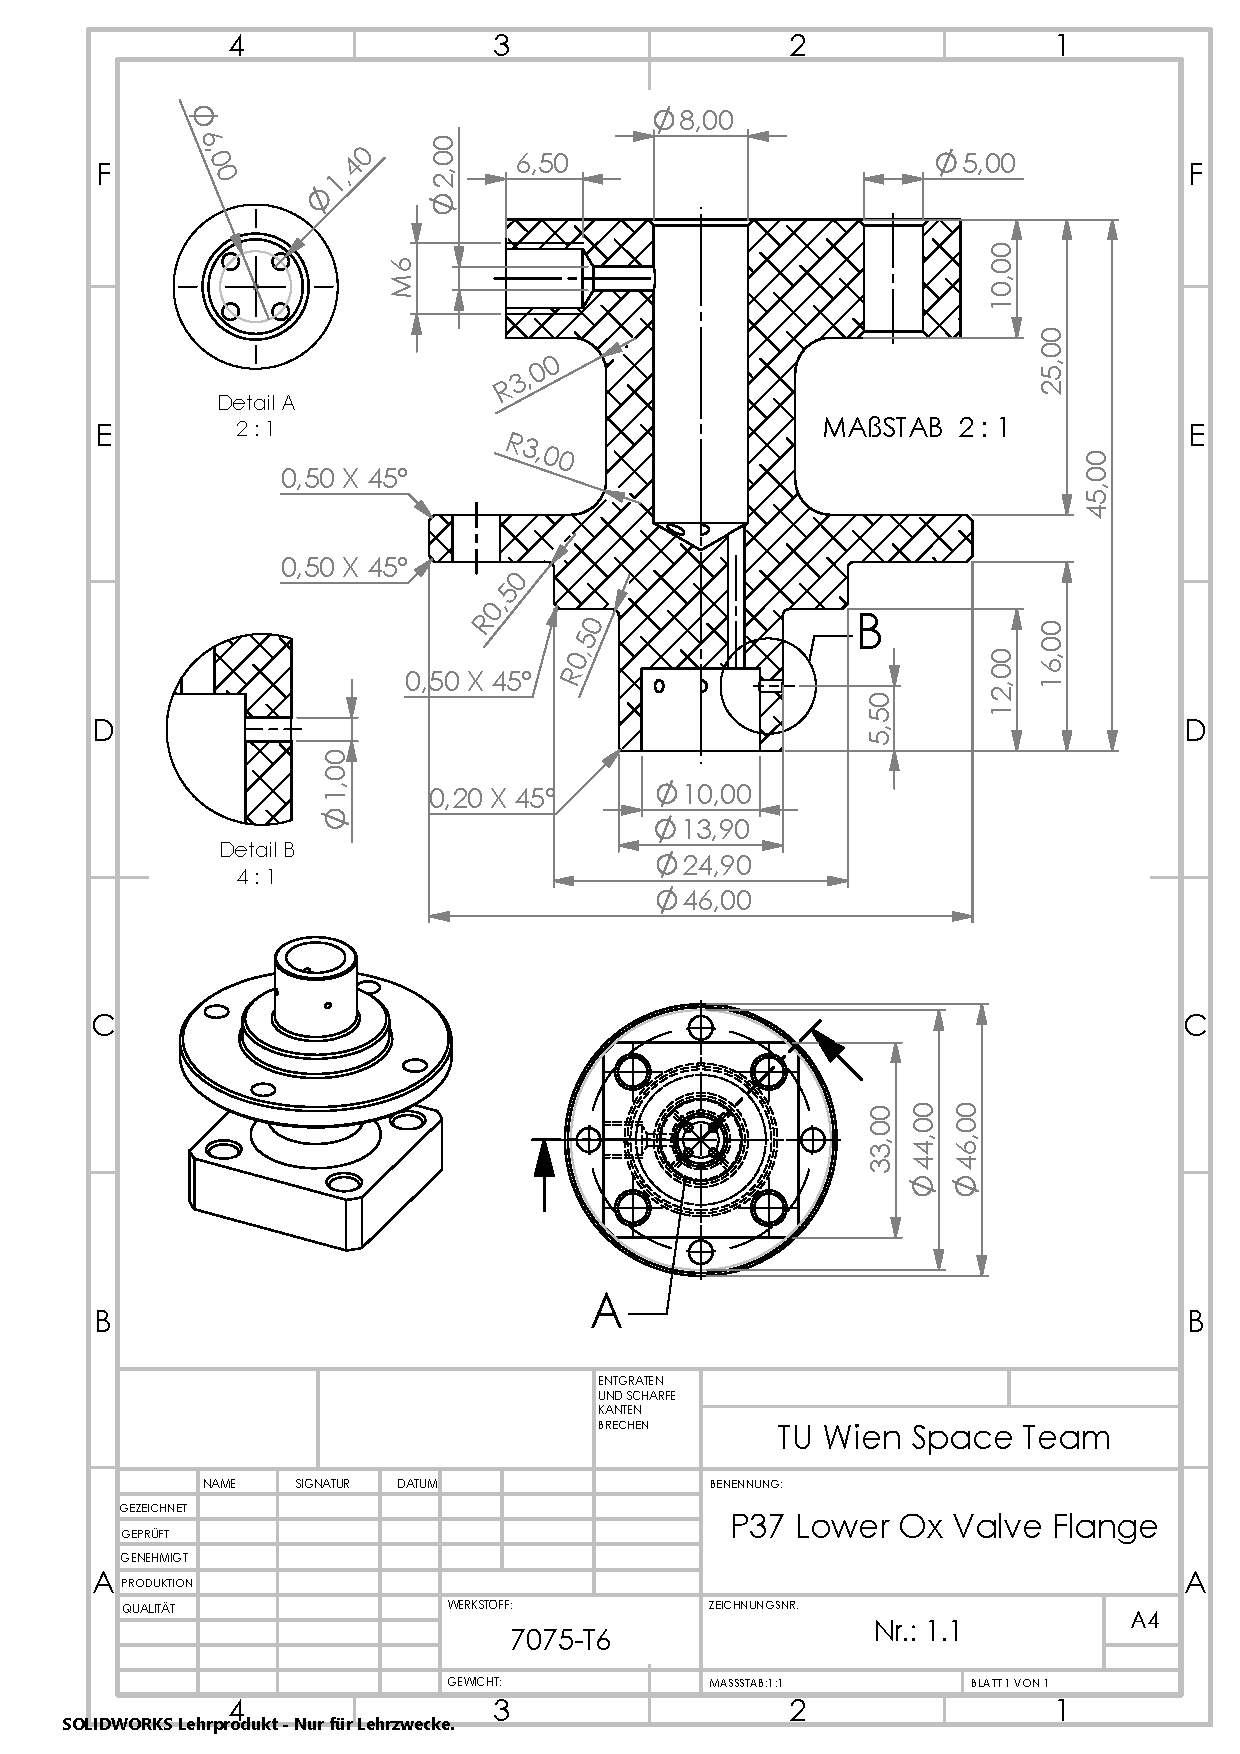
\includepdf[pages=-]{Appendices/P37_Injector_Lower_Ox_Valve_Flange.pdf}
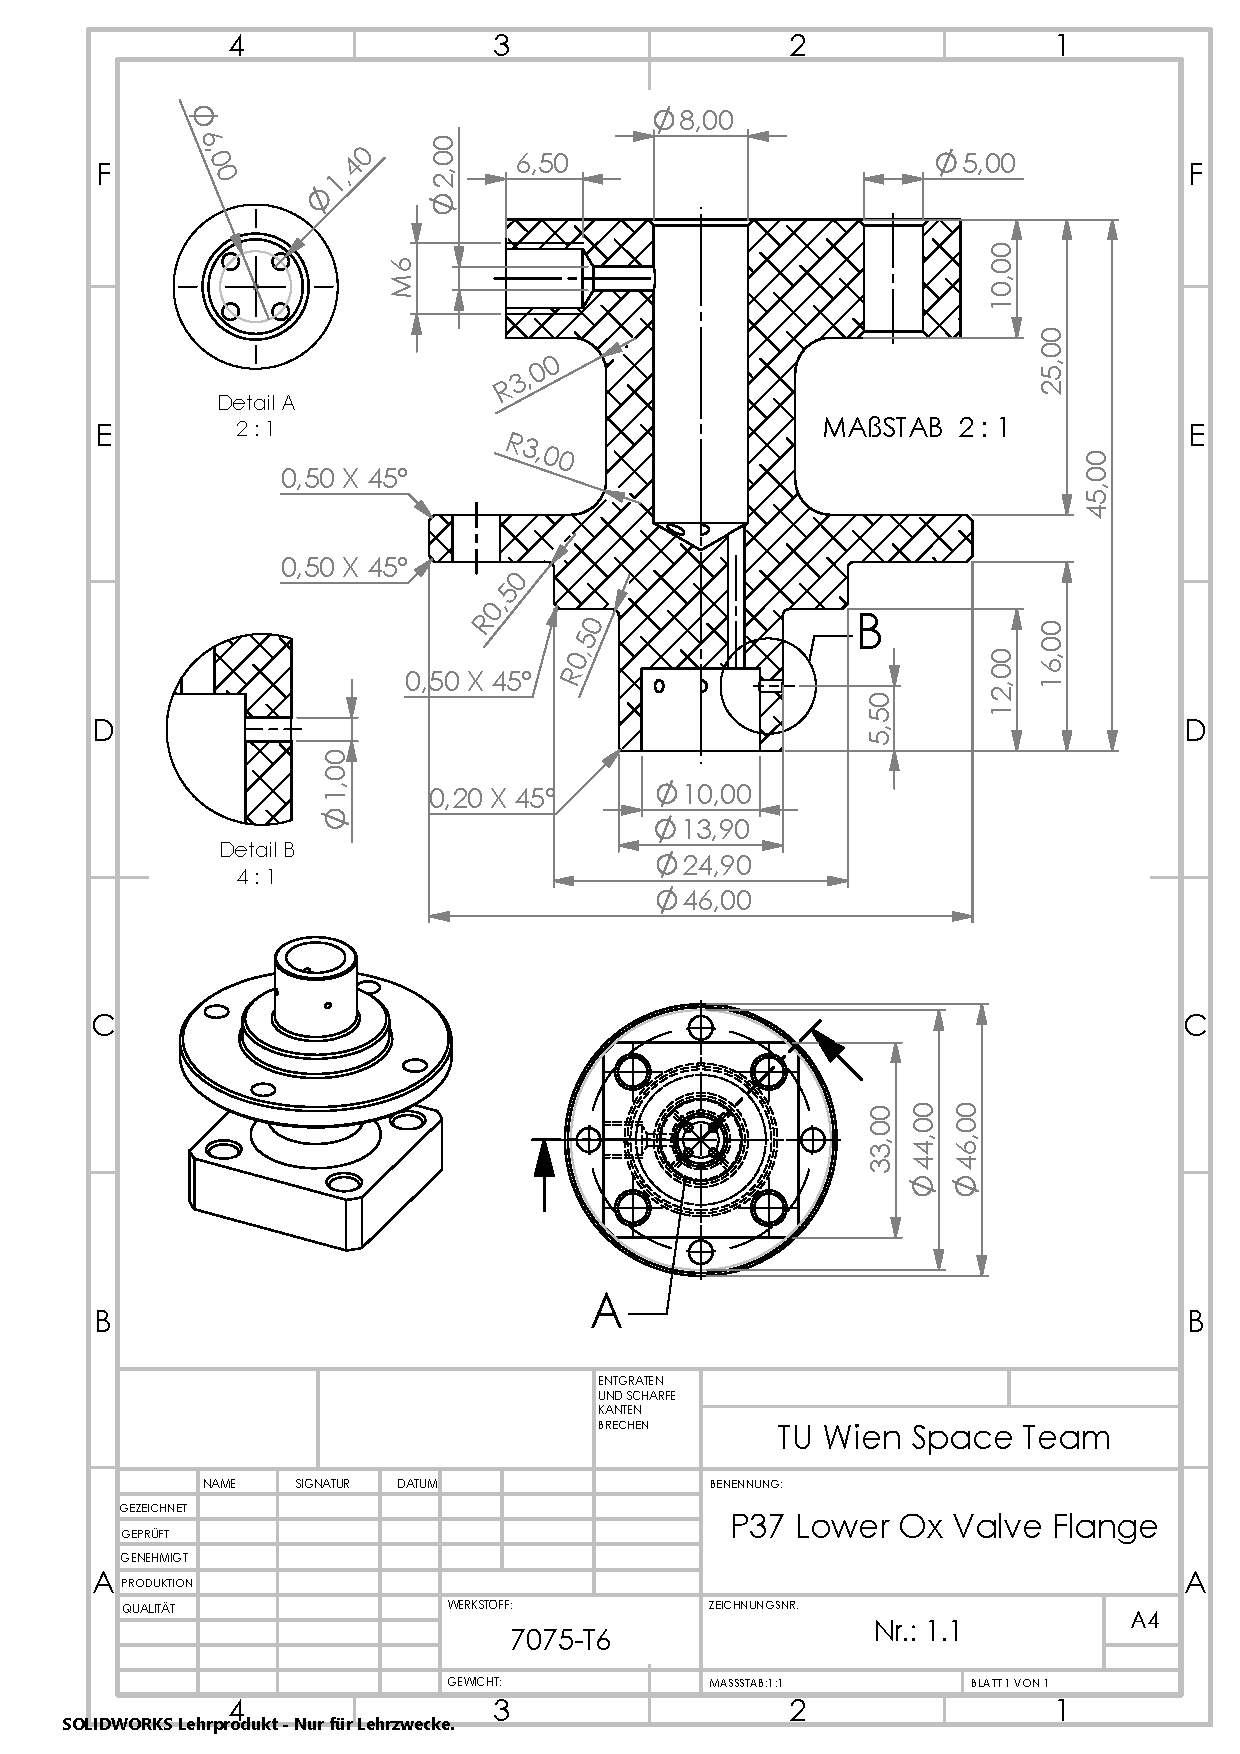
\includepdf[pages=-]{Appendices/P37_Lower_Ox_Valve_Flange.pdf}
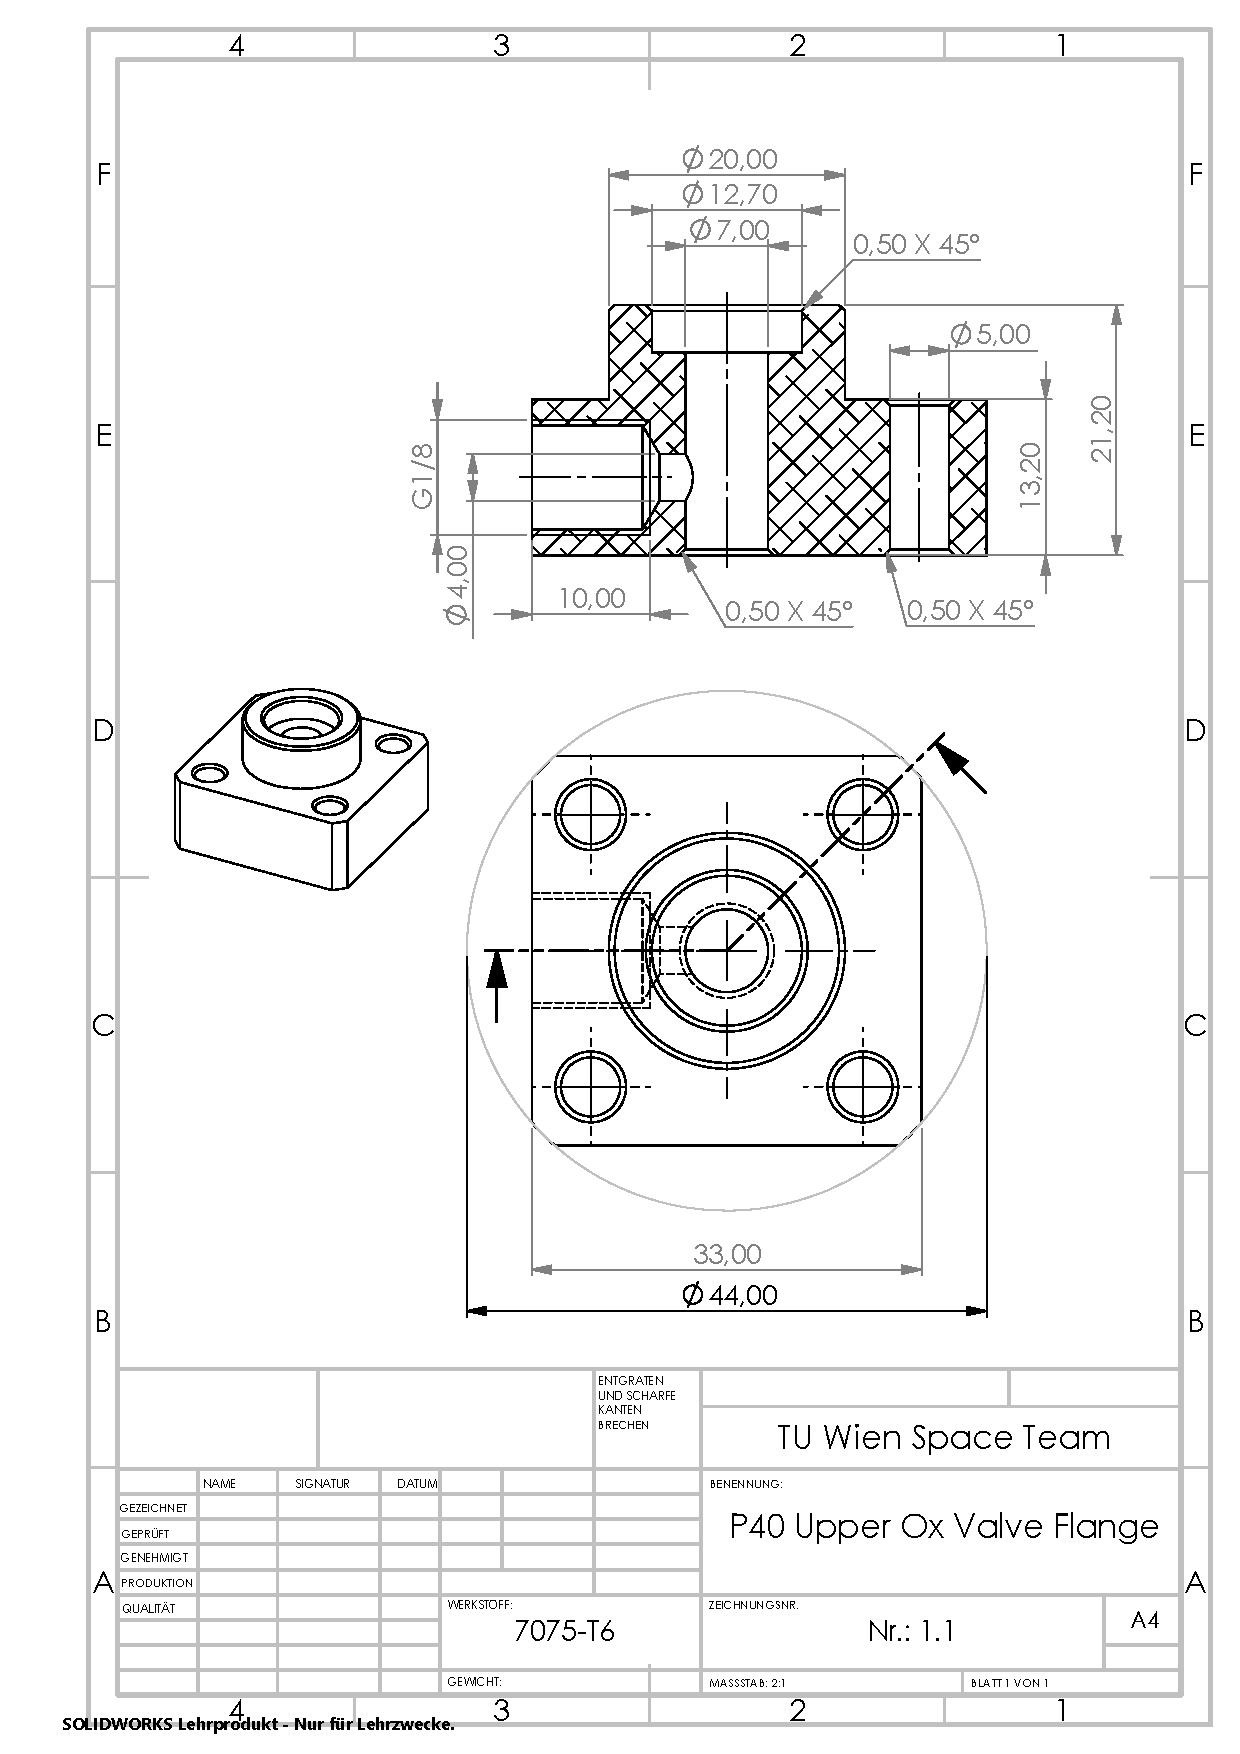
\includepdf[pages=-]{Appendices/P40_Upper_Ox_Valve_Flange.pdf}
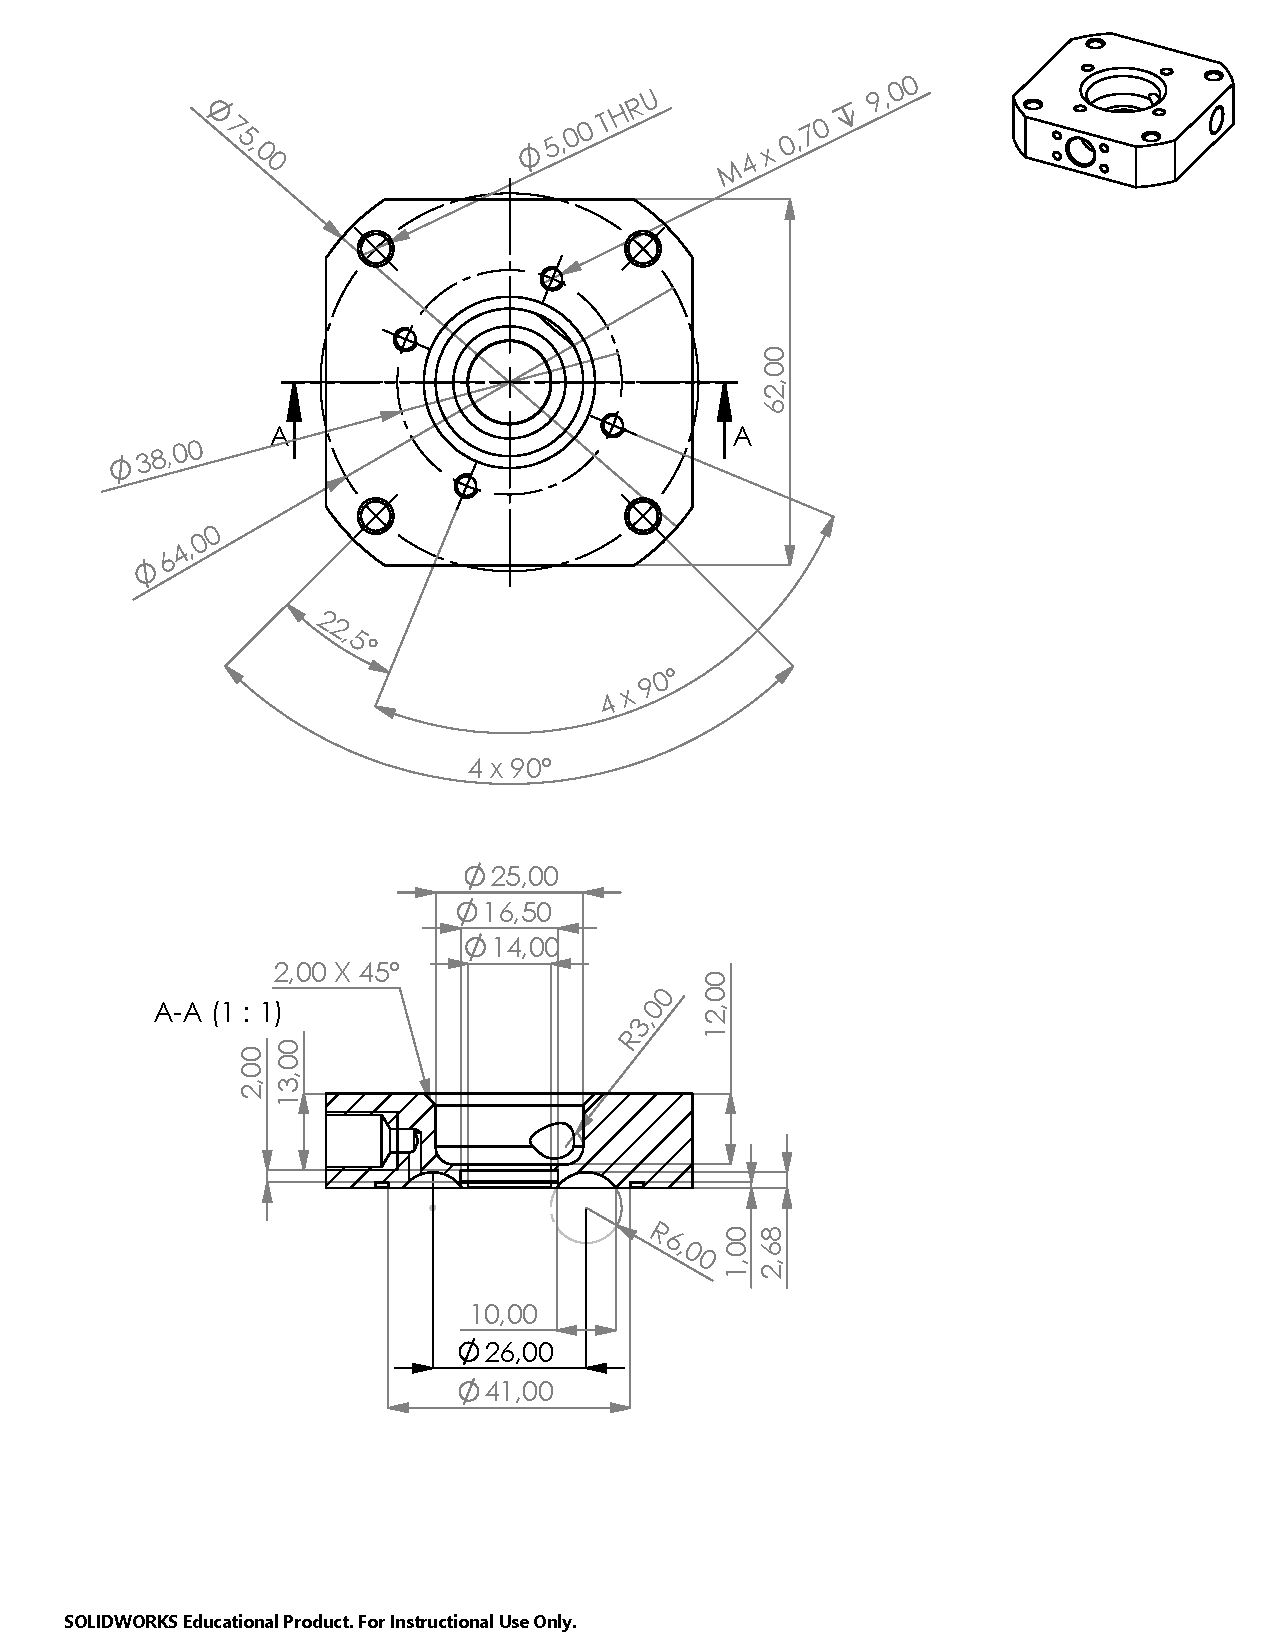
\includepdf[pages=-]{Appendices/EngineHead.pdf}
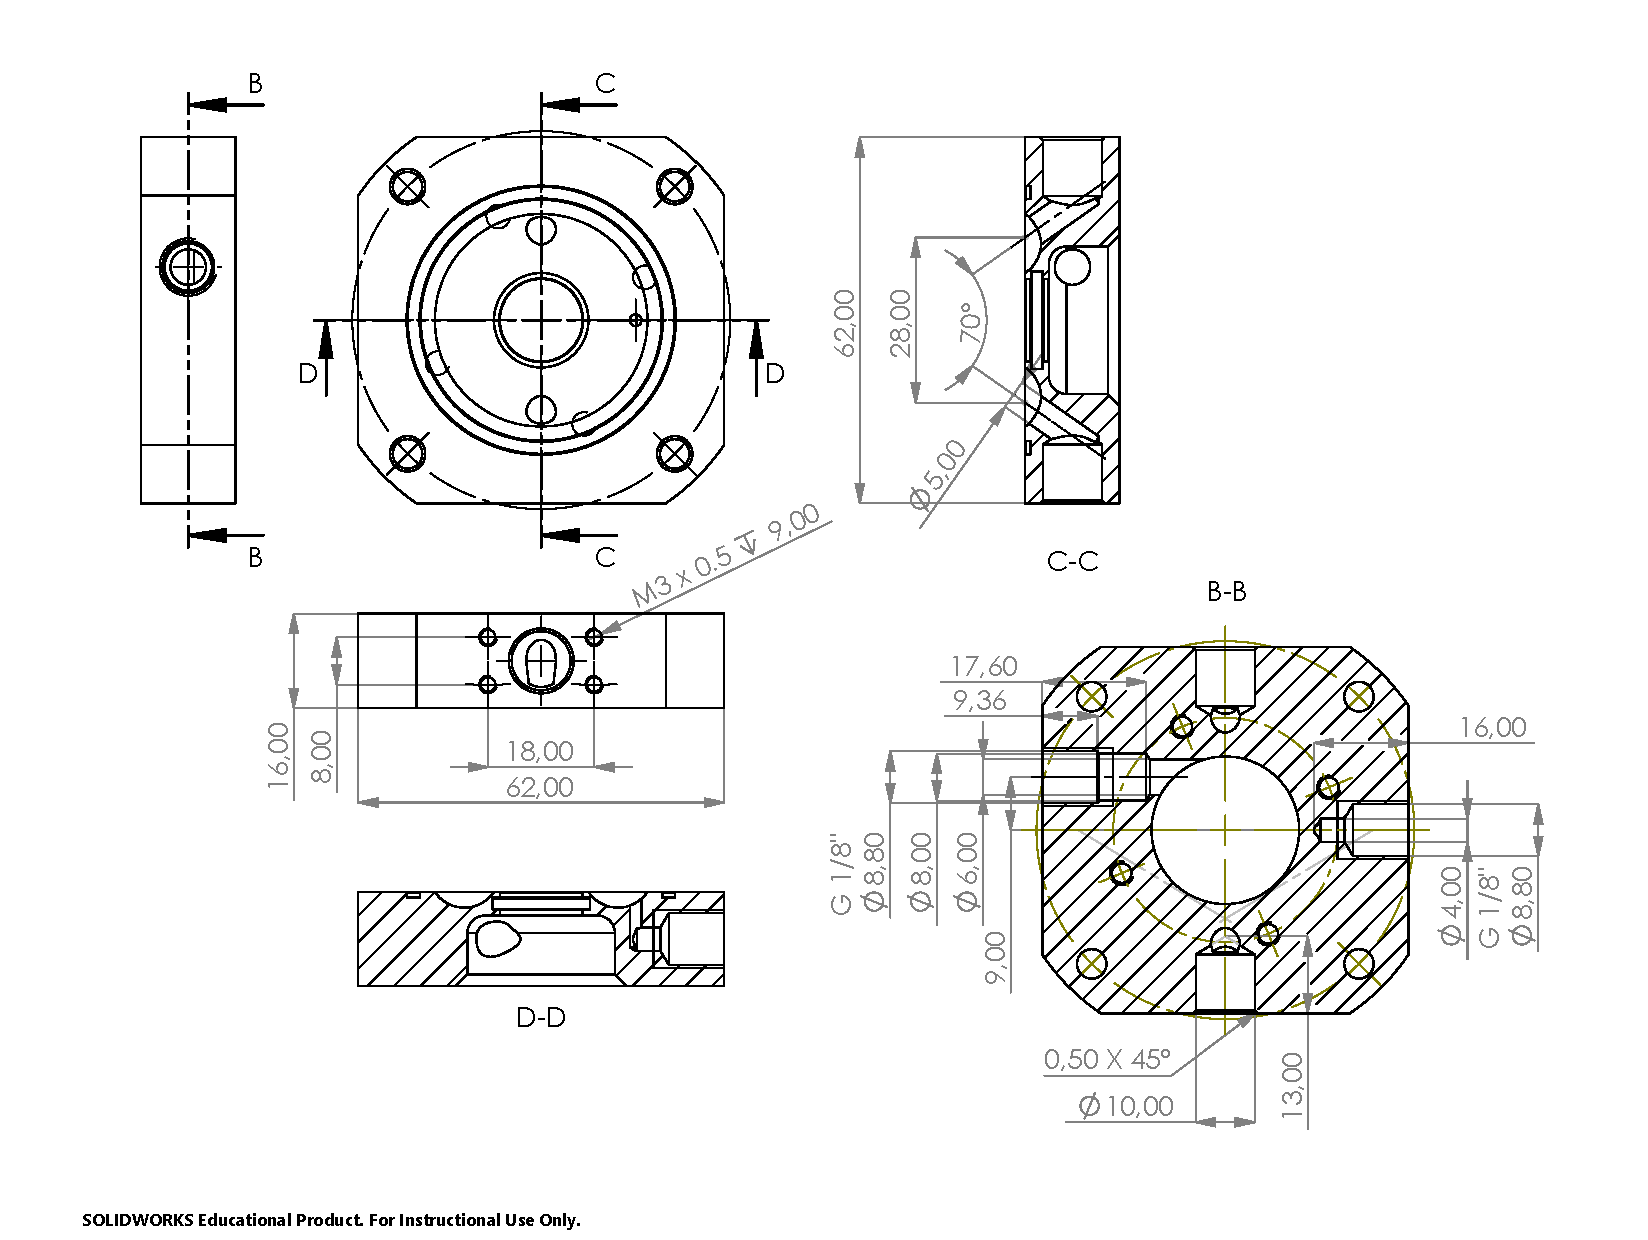
\includepdf[pages=-]{Appendices/EngineHead2.pdf}

%from here on out optional
\section{Detailed Software Architecture}\label{sec:software}

\begin{figure}[h]
    \centering
    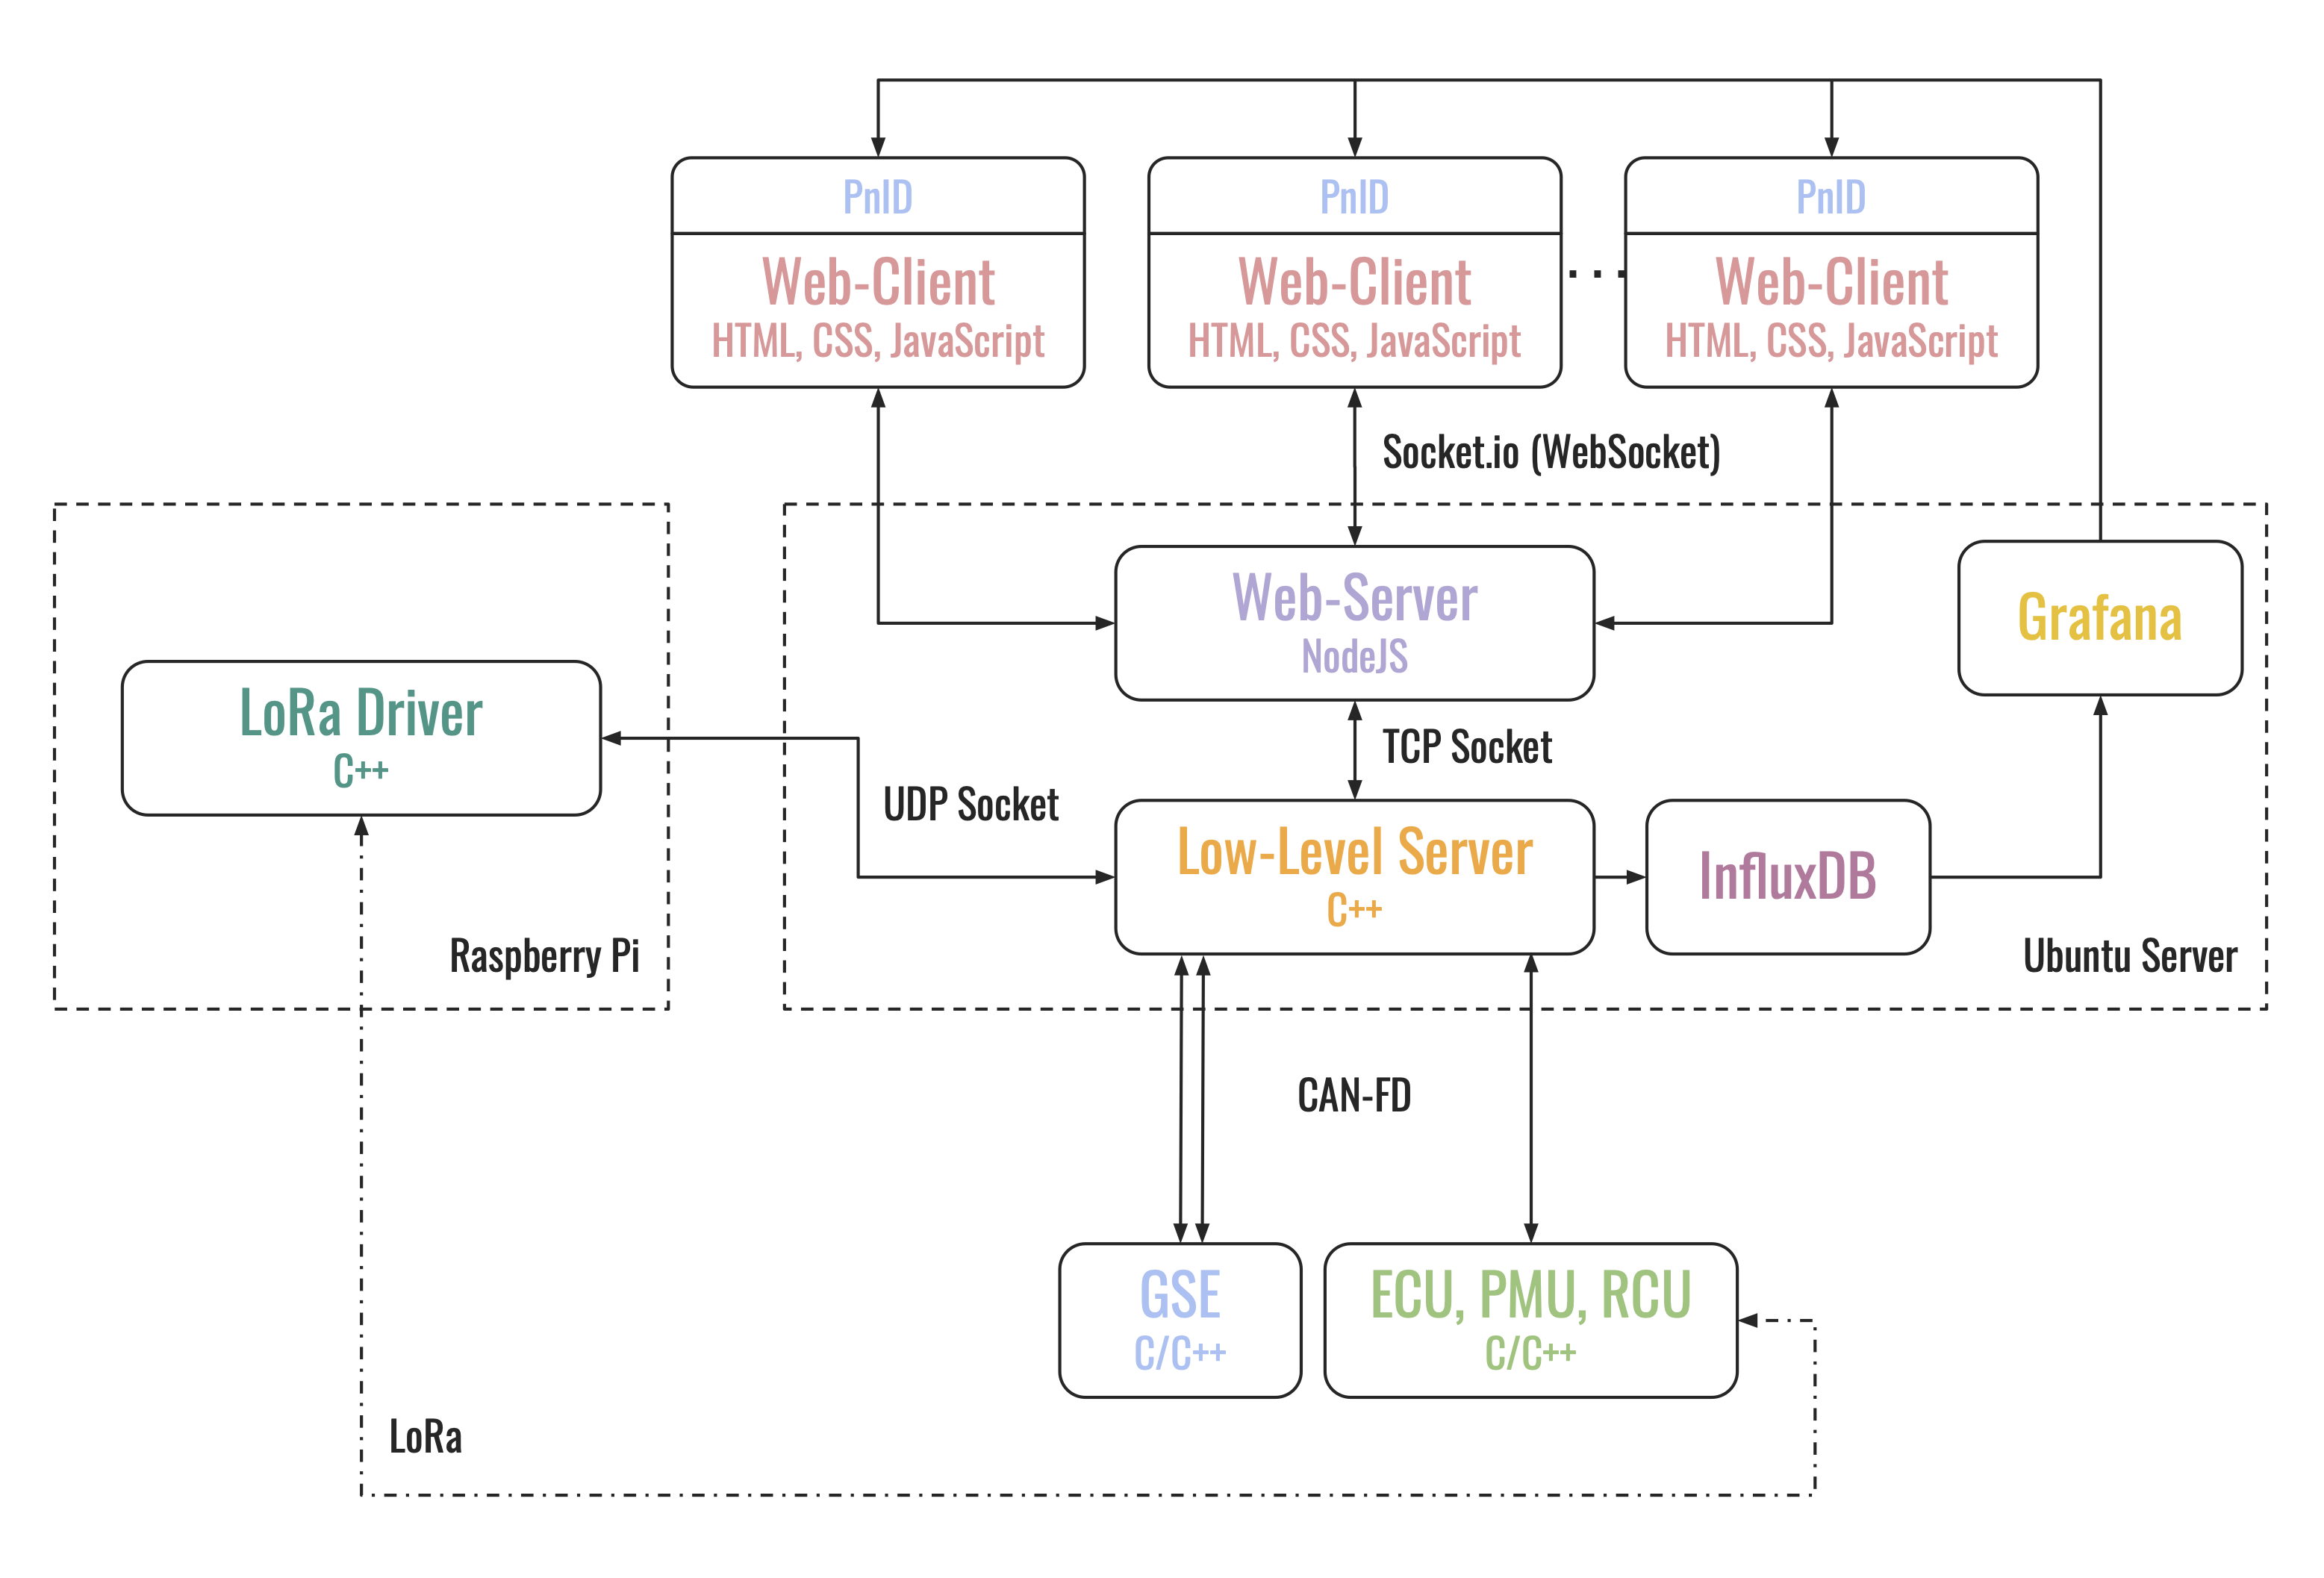
\includegraphics[width=0.7\textwidth]{Appendices/Software Architecture.png}
    \caption{Software Architecture}
    \label{fig:software}
\end{figure}


\subsection{Mission Control} %Markus
Mission Control consists of a PC or Laptop running a Web-Application (Web-Client) inside a Web-Browser. It manages the communication between the Operator and the Rocket as well as the Ground Support Equipment. The Web-Client displays all measured data and actuators in a self developed interactive Piping and Instrumentation Diagram (P\&ID/PnID). 
Every value for each P\&ID element gets validated. When out of range, it is
signalled by changing colour. This way, the operator doesn't have to check
each number in detail but rather only has to watch for color changes, which is much
more apparent.

\subsection{Ubuntu Server}

The Ubuntu Server uses a PCIe CAN bus extension card with four CAN bus ports.
It is responsible for communication with the Hardware, i.e. GSE, ECU, RCU and PMU.
Mission Control interfaces with the Hardware via a self developed software as 
depicted in figure \ref{fig:software}. The connection from the server to Mission Control can either be made by a long Ethernet cable or a directed radio link depending on the necessary safety distance of MC from the pad. 

\paragraph{Low-Level Server}

Written in C++ it is responsible for managing CAN and other time critical tasks such as logging and processing sensor data.

\paragraph{Web-Server}

Uses NodeJS to host the Web-Clients and synchronize data between them.

\paragraph{InfluxDB and Grafana}

InfluxDB is a time series based database for logging sensor data and user inputs. Grafana is used for real time plots and gauges on the Web-Client. It is also used for
post-launch procedures.

\subsection{LoRa Raspberry Pi}

To communicate with the rocket during flight, LoRa is used. A self developed
LoRa transceiver shield is connected to a Raspberry Pi which processes and 
transmits the messages over UDP to the Ubuntu Server. There it gets processed
like a normal CAN Message.
